\documentclass[hidelinks]{ipn}
\usepackage{ipnstyle}
\usepackage{lipsum}
\usepackage{graphicx}
\usepackage{float}
\usepackage{caption}
\usepackage{subcaption}
\usepackage{bookmark}
\usepackage{hyperref}
\usepackage{minted}
% \usepackage{cite}

\usepackage{tikz, lipsum, lmodern}
\usepackage[most]{tcolorbox}
\usepackage{etoolbox}  % Añade esta línea
\usepackage{microtype}  % Mejora la justificación y tipografía
\usepackage{ragged2e}  % Añade esta línea en el preámbulo
\usepackage{parskip}
\usepackage{changepage} % en el preámbulo
\setlength{\parindent}{0pt}
% Añade esta línea antes de \begin{document}
\let\cleardoublepage\clearpage
\setlength{\emergencystretch}{3em}
\tolerance=9999
\AtBeginDocument{\justifying}

\makeatletter
\makeatother

\author{José Emiliano Carrillo Barreiro\\
        José Ángel Robles Otero}
\title{Modelo para representar comportamientos gravitacionales con dos cuerpos}
\schoolname{Escuela Superior de Cómputo}
\degree{Maestría en Ciencias de la Computación}
\advisor{Dr.\ Cesar Hernández Vasquez}
\coadvisor{Dr.\ Mauricio Olguín Carbajal}
\academicyear{\today}

\hypersetup{
    colorlinks=false,
    pdfauthor={Your Name},
    pdftitle={Modelo para representar comportamientos gravitacionales con dos cuerpos},
    pdfsubject={Thesis},
    pdfkeywords={keyword1, keyword2, keyword3}
    pdfproducer={Latex with hyperref},
    pdfcreator={pdflatex}
}

\addbibresource{./references.bib}
\pagestyle{headings}

% ========= DEFINICIONES DE COLORES

\begin{document}
\justifying%
\frontmatter
    \maketitle
    \begin{titlepage}
    \begin{center}
        % Logo and Institute Name placement
        \raisebox{0.0\height}{
        \begin{adjustbox}{max width=1.2\linewidth, right}
          \begin{minipage}[c]{0.5\linewidth}
            \centering
           \raisebox{0.0\height}{\includegraphics[width=0.5\linewidth]{img/logo-ipn.png}}
          \end{minipage}\hfill
          \begin{minipage}[c]{1.5\linewidth}
            \centering
            {\fontsize{28}{30}\selectfont\textsc{Instituto Politécnico Nacional}}\\[2mm]
            {\fontsize{24}{26}\selectfont\textsc{Escuela Superior de Cómputo}}\\[2mm]
            {\fontsize{20}{22}\selectfont\textsc{Subdirección Académica}}
        \end{minipage}
        \hfill
          \begin{minipage}[c]{0.5\linewidth}
            \centering
            \raisebox{0.0\height}{\includegraphics[width=0.8\linewidth]{img/EscudoESCOM.png}}
          \end{minipage}
        \end{adjustbox}}

        \begin{adjustwidth}{-2.5cm}{}
            \begin{center}
                \begin{tabular}{c@{\hspace{8cm}}c}
                    No.\ de TT:\ 2025-B065 &
                    \today
                \end{tabular}\\
                \vspace{0.55cm}
                \textbf{Documento técnico} \\
                
                \vspace{0.5cm}
                
                % Title
                \begin{minipage}{0.8\textwidth}
                    \centering
                    {\fontsize{16}{16}\selectfont\textbf{``Modelo para representar comportamientos gravitacionales con dos cuerpos''\\}}
                \end{minipage}
                
                \vspace{0.3cm}
                
                % Presentan
                {\fontsize{16}{16}\selectfont\textit{Presentan:}} \\
                \vspace{0.25cm}
                % Authors (names in alphabetical order by last name)
                {\fontsize{14}{14}\selectfont\textbf{
                José Emiliano Carrillo Barreiro.\footnote{\href{mailto:carrillobarjosee@gmail.com}{carrillobarjosee@gmail.com}}\\
                José Ángel Robles Otero.\footnote{\href{mailto:robles.otero.jose.angel@gmail.com}{robles.otero.jose.angel@gmail.com}}}
                }
                \vspace{0.5cm}
                
                % Directors
                {\fontsize{14}{14}\selectfont\textsc{Directores:\\}}
                
                \vspace{10pt}
                
                % Director names
                {\fontsize{14}{14}\selectfont\textbf{Dr.\ Cesar Hernández Vasquez\\}}
                
                \vspace{5pt}
                
                % Co-director (if applicable)
                {\fontsize{14}{14}\selectfont\textbf{Dr.\ Mauricio Olguín Carbajal}}
                
                \vspace{0.5cm}
                
                % Abstract
                \begin{minipage}{\textwidth}
                    \begin{center}
                        \textbf{Resumen:}\\[0.3cm]
                    \end{center}
                    {\fontsize{12}{12}\selectfont
                    En los últimos años, la elaboración de entornos virtuales complejos, como \textit{REBOUND}, \textit{Universe sandbox}, \textit{Stellarium} y \textit{Celestia}, han experimentado un crecimiento exponencial en sus capacidades. Más, cuando se habla de implementar mejoras en la precisión y escalabilidad dentro de sistemas de \textit{n}-cuerpos celestes, por ejemplo, la simulación de nacimientos de galaxias, todavía existen dificultades, ya que, actualmente, los modelos que los simulan no permiten introducir cambios en los parámetros de los cuerpos durante su ejecución, parámetros como la velocidad, posición y masa del cuerpo, lo que impide contar con escenarios más fidedignos a los comportamientos  físicos dentro de sistemas de $n$-cuerpos atípicos. En este proyecto, se propone solucionar este problema mediante la construcción de un modelo que permita realizar cambios al parámetro más significativo del  sistema, compuesto por dos cuerpos, en tiempo de ejecución, implementando técnicas como el método multipolar rápido (FMM, por sus siglas en inglés, \textit{Fast Multipole Method}), el \textit{algoritmo de Barnes-Hut} y algoritmos bioinspirados. La solución que se desarrolle podría usarse para simular comportamientos físicos dentro de entornos virtuales.\\

                     \textbf{Palabras clave: } Modelado y Simulación de sistemas, problema de los $n$-cuerpos, Mecánica Celeste, y Algoritmos Bioinspirados.}
                \end{minipage}
                
                \vspace{0.7cm}
                
                % Date
                \textbf{\large Fecha: \today}
            \end{center}
        \end{adjustwidth}
    \end{center}
\end{titlepage}
    \filright%
\begin{minipage}{\textwidth}
    \filright%
    \centering
    \begin{tcolorbox}[enhanced,attach boxed title to top center={yshift=-3mm,yshifttext=-1mm},
      colback=blue!5!white,colframe=blue!75!black,colbacktitle=red!80!black,
      title=\textbf{Advertencia},fonttitle=\bfseries,
      boxed title style={size=small,colframe=red!50!black} ]
    \textit{“Este documento contiene información desarrollada por la Escuela
    Superior de Cómputo del Instituto Politécnico Nacional, a partir de datos y
    documentos con derecho de propiedad y por lo tanto, su uso quedará
    restringido a las aplicaciones que explícitamente se convengan.”}\\

    La aplicación no convenida exime a la escuela su responsabilidad técnica y
    da lugar a las consecuencias legales que para tal efecto se determinen.\\

    Información adicional sobre este reporte técnico podrá obtenerse en:\\

    La Subdirección Académica de la Escuela Superior de Cómputo del Instituto
    Politécnico Nacional, situada en Av. Juan de Dios Bátiz s/n Teléfono: 57296000, extensión 52000.
    \end{tcolorbox}
\end{minipage}
    \input{frontmatter/00-Advertencia}
    \chapter{Resumen.}
\justifying
En los últimos años, la elaboración de entornos virtuales complejos, 
como \textit{REBOUND}, \textit{Universe sandbox}, \textit{Stellarium} y \textit{Celestia}, 
han experimentado un crecimiento exponencial en sus capacidades. Más, cuando se habla de 
implementar mejoras en la precisión y escalabilidad dentro de sistemas de \textit{n}-cuerpos celestes, 
por ejemplo, la simulación de nacimientos de galaxias, todavía existen dificultades, ya que, actualmente, 
los modelos que los simulan no permiten introducir cambios en los parámetros de los cuerpos durante su ejecución, 
parámetros como la velocidad, posición y masa del cuerpo, lo que impide contar con escenarios más fidedignos a los 
comportamientos  físicos dentro de sistemas de $n$-cuerpos atípicos. En este proyecto, se propone solucionar este 
problema mediante la construcción de un modelo que permita realizar cambios al parámetro más significativo del  sistema, 
compuesto por dos cuerpos, en tiempo de ejecución, implementando técnicas como el método multipolar rápido (FMM, por sus siglas en inglés, 
\textit{Fast Multipole Method}), el \textit{algoritmo de Barnes-Hut} y algoritmos bioinspirados. La solución que se desarrolle podría usarse 
para simular comportamientos físicos dentro de entornos virtuales.\\

\chapter{Abstract.}
\lipsum[1-3]
    \chapter{Agradecimientos.}
El presente trabajo terminal, documentado en este informe técnico, no habría sido posible sin el invaluable apoyo, la guía y la inspiración de numerosas personas a lo largo de nuestra trayectoria académica. A todos ellos, expresamos nuestro más profundo y sincero agradecimiento.

En primer lugar, deseamos reconocer a nuestros directores, el Dr.\ Cesar Hernández Vásquez y el Dr.\ Mauricio Olguín Carbajal, por su dedicación, paciencia y valioso apoyo intelectual durante este proceso. Su orientación especializada, sus críticas constructivas y su constante motivación han sido pilares fundamentales en el desarrollo de la investigación y la propuesta de solución planteada en este proyecto. Sin su confianza y disposición para compartir su conocimiento, esta primera presentación de resultados no habría alcanzado su forma actual.

Asimismo, extendemos nuestra gratitud a los miembros del comité sinodal, la Dra. Yesica Sonia Flores Meraz, el M. en C. Jesús Alfredo Martínez Nuño y el Dr.\ Genaro Juárez Martínez, por su tiempo, esfuerzo y compromiso al evaluar este trabajo terminal. Sus comentarios y sugerencias han enriquecido significativamente la calidad de esta investigación y seguirán siendo esenciales para su mejora.

De manera especial, agradecemos a la Dra. Lorena Chavarría Báez por su apoyo incondicional en el planteamiento del protocolo y la delimitación del proyecto. Sus aportaciones y sugerencias fueron cruciales para afinar el enfoque de esta investigación, contribuyendo a la profundidad y claridad que caracterizan el trabajo aquí presentado.

Igualmente, queremos destacar la colaboración de los Dr.\ Daniel Molina Pérez y M. en C. José Alberto Torres León, quienes, en su rol de consultores expertos, revisaron el propósito, los objetivos y el desarrollo de este proyecto. Su retroalimentación, validada mediante el “juicio de experto”, junto con sus valiosos comentarios, nos permitió perfeccionar las técnicas y la calidad de este informe.

Por último, pero no menos importante, rendimos homenaje a nuestras familias por su amor incondicional, paciencia y sacrificios a lo largo de este arduo camino. Su respaldo constante ha dado un significado especial a esta presentación.
A través de esta primera parte del trabajo terminal, hemos enfrentado desafíos que nos han permitido crecer tanto personal como académicamente. Este proceso nos ha revelado nuevas dimensiones del conocimiento, así como la resiliencia y determinación que habitan en nosotros. A todos quienes nos han acompañado con su apoyo, guía e inspiración, les debemos una parte esencial de este logro inicial. Gracias por todo.

    \tableofcontents
    \listoffigures
    \listoftables
    \listofalgorithms%

\mainmatter%
    %\include{chapters/chapter01}
    %\include{chapters/chapter02}
    \chapter{Introducción}\label{ch:Introduccion}
    \section{Antecedentes}
El desarrollo de simulaciones de \textit{n}-cuerpos ha sido ampliamente investigado con el objetivo de mejorar su capacidad para modelar fenómenos complejos en entornos como la colisión de galaxias y la evolución de sistemas planetarios. Sin embargo, una limitación crítica es la incapacidad de ajustar los parámetros de los cuerpos durante la ejecución de la simulación, lo que afecta la representación precisa de eventos masivos como colisiones en las simulaciones disponibles.

El problema de los \textit{n}-cuerpos\footnote{El problema de \textit{n}-cuerpos se refiere al estudio del movimiento e interacción gravitacional de varios cuerpos bajo sus influencias mutuas. En la sección~\ref{sec:n-body_problem} se profundiza a fondo el termino.} ha sido uno de los desafíos más complejos en la mecánica celeste, desde los trabajos pioneros de Newton en el siglo XVII.\ Si bien el problema de los dos cuerpos tiene una solución analítica exacta bajo ciertas condiciones, cuando se introducen factores adicionales, se requieren métodos numéricos avanzados para mejorar la precisión de las simulaciones.

Avances como el método multipolar rápido (FMM, por sus siglas en inglés, \textit{Fast Multipole Method})\footnote{El FMM es un algoritmo que optimiza el cálculo de interacciones entre partículas distantes en sistemas físicos, como los gravitacionales, agrupando partículas y aproximando su influencia colectiva, lo que reduce la complejidad computacional de \(O(n^2)\) a \(O(n)\) o \(O(n \log n)\).} y el algoritmo de Barnes-Hut\footnote{El algoritmo de Barnes-Hut es una técnica de simulación de \textit{n}-cuerpos que aproxima las fuerzas gravitacionales al agrupar cuerpos distantes en una misma región del espacio, representándolos como una única masa, lo que reduce la complejidad computacional de \(O(n^2)\) a \(O(n \log n)\).} han optimizado las simulaciones de \textit{n}-cuerpos al reducir la complejidad computacional en el cálculo de las interacciones gravitacionales. Sin embargo, la falta de capacidad para ajustar dinámicamente las propiedades de los cuerpos durante la ejecución sigue siendo una limitación en la representación realista de eventos astronómicos.

Estudios recientes han introducido herramientas y enfoques que podrían mejorar las simulaciones de \textit{n}-cuerpos, como el uso de árboles cuádruples y octales para la representación geométrica y la aplicación de inteligencia artificial en las simulaciones moleculares que podrían inspirar nuevas técnicas en simulaciones celestes. Además, se ha demostrado la eficacia de integradores simplécticos\footnote{Los integradores simplécticos son métodos numéricos utilizados para resolver ecuaciones diferenciales en sistemas dinámicos conservando las propiedades geométricas del sistema, como la conservación de la energía a largo plazo, lo que los hace especialmente adecuados para simular interacciones físicas, como las gravitacionales, en sistemas de \textit{n}-cuerpos.} para garantizar la estabilidad de las simulaciones durante colisiones y la paralelización para mejorar la eficiencia en simulaciones masivas.
    \section{Planteamiento del problema}
Las simulaciones de sistemas de \textit{n}-cuerpos celestes han sido una herramienta fundamental en la astronomía y la mecánica celeste para estudiar la evolución de sistemas planetarios, la dinámica estelar y la interacción gravitacional a gran escala. Sin embargo, una limitación crítica en los modelos actuales es la imposibilidad de modificar dinámicamente los parámetros de los cuerpos durante la ejecución de la simulación. En la mayoría de los simuladores, estos parámetros, como la masa, la energía del sistema, la posición y el tiempo de existencia de los cuerpos se definen antes de la ejecución, impidiendo la representación precisa de eventos atípicos o transitorios, como colisiones de galaxias, acreción de materia en discos protoplanetarios o cambios de masa en estrellas variables.

Uno de los problemas más importantes derivados de esta limitación es la incapacidad de ajustar la masa de los cuerpos celestes durante el lapso de duración de la simulación. En eventos como fusiones de agujeros negros o estrellas en procesos de acreción, la masa de los cuerpos cambia significativamente a lo largo del tiempo, alterando la evolución del sistema. Sin la posibilidad de modificar este parámetro de manera dinámica, los modelos actuales ofrecen solo aproximaciones estáticas que no reflejan con precisión la naturaleza de estos fenómenos.

Además, el rendimiento computacional también representa un desafío. La simulación de \textit{n}-cuerpos es un problema computacionalmente costoso, ya que la cantidad de interacciones a calcular crece cuadráticamente con el número de cuerpos ($O~(n^2)$), lo que hace que las simulaciones a gran escala sean prohibitivas en términos de tiempo de ejecución y recursos computacionales. Métodos como el algoritmo de Barnes-Hut y el método multipolar rápido han sido desarrollados para mitigar este problema reduciendo la cantidad de cálculos directos, pero no abordan la falta de flexibilidad en la modificación de parámetros en tiempo real.

En este contexto, la incapacidad de modificar parámetros dinámicamente en simulaciones de \textit{n}-cuerpos afecta no solo a la estabilidad del sistema representado durante la simulación, respecto a los fenómenos astronómicos internos del sistema; sino también la capacidad de realizar simulaciones interactivas, algo que podría tener aplicaciones en la enseñanza, la exploración espacial y la industria del entretenimiento. La ausencia de modelos que permitan esta flexibilidad limita el alcance de las simulaciones actuales y plantea la necesidad de desarrollar enfoques más adaptativos y eficientes.
    \section{Propuesta de solución}

La solución propuesta se basa en el desarrollo de un modelo que permite la modificación dinámica de parámetros durante la simulación, lo que representa una mejora significativa con respecto a los simuladores tradicionales, que requieren reconfiguraciones antes de cada ejecución. Este modelo integrará técnicas avanzadas para optimizar el cálculo de interacciones gravitacionales y garantizar la estabilidad de la simulación.

Para lograrlo, se emplearán distintos métodos de cálculo sobre fuerzas gravitacionales y cálculos de colisión. Respecto a los cálculos de fuerzas gravitacionales, uno de los elementos plausibles a integrar es el método multipolar rápido (FMM) y el algoritmo de Barnes-Hut, ambos ampliamente utilizados para reducir la complejidad computacional en simulaciones de \textit{n}-cuerpos sin comprometer la precisión.\ Estas técnicas permiten agrupar cuerpos en estructuras jerárquicas, disminuyendo el número de cálculos directos y mejorando la eficiencia del sistema.

Además, la implementación de algoritmos bioinspirados, como la optimización por enjambre de partículas (PSO) y algoritmos genéticos (AGs), permitirá el ajuste dinámico de los parámetros de los cuerpos celestes, garantizando un comportamiento estable incluso en escenarios de colisión o interacciones complejas. Estas estrategias facilitarán la identificación y ajuste de valores óptimos sin necesidad de intervención manual, lo que hará que la simulación sea más adaptable a eventos inesperados.

El modelo se diseñará para ser escalable, permitiendo la modificación de los parámetros, conjunto de parámetros que solo involucra a la masa de los cuerpos dada las limitaciones de tiempo para el trabajo terminal, de hasta dos cuerpos celestes, con la posibilidad de extenderse a más cuerpos en implementaciones futuras. Su integración con entornos virtuales como Unreal Engine o motores de simulación especializados permitirá su aplicación en campos como la educación, los videojuegos y la industria aeroespacial; dicha implementación se deja para mejoras futuras al proyecto.

Para garantizar un rendimiento eficiente, el modelo se desarrollará optimizado para ejecutarse en hardware de gama media, como procesadores multinúcleo con al menos 16 GB de RAM.\ Esto asegurará que la solución sea accesible sin requerir infraestructuras de alto rendimiento, ampliando su potencial uso en distintos ámbitos.

Esta combinación de técnicas avanzadas y adaptabilidad en tiempo real establece una base innovadora para el desarrollo de simulaciones gravitacionales más dinámicas, eficientes y versátiles, superando las limitaciones de los modelos preconfigurados actuales.
    \section{Objetivo general}
Desarrollar un modelo teórico para la simulación del problema de dos cuerpos que permita la modificación dinámica de la masa, mejorando la precisión en la representación de sus interacciones gravitacionales y eventos asociados.
\subsection{Objetivos específicos}
\begin{itemize}
    \item Desarrollar el módulo de simulación para la integración del método multipolar rápido (FMM) y el algoritmo de Barnes-Hut.
    
    \item Desarrollar el módulo de optimización para ajustar dinámicamente la configuración del sistema con algoritmos bioinspirados.

    \item Desarrollar la implementación del modelo de simulación dinámica de interacciones gravitatorias entre dos cuerpos.

    \item Desarrollar el módulo de visualización para representar gráficamente la evolución del sistema en un número limitado de iteraciones.

    \item Desarrollar una interfaz básica para la modificación de parámetros y la visualización de resultados.
\end{itemize}
    \section{Justificaión}
Este proyecto es relevante porque introduce un enfoque innovador en la simulación de sistemas gravitacionales al permitir la modificación dinámica de parámetros, superando las limitaciones de los modelos tradicionales. La elección de algoritmos avanzados, como el método multipolar rápido (FMM) y el algoritmo de Barnes-Hut, garantiza un equilibrio entre precisión y eficiencia computacional, lo que permite su aplicación en escenarios más complejos sin un costo computacional excesivo. Además, la implementación de técnicas de optimización bioinspiradas ofrece un método adaptable para ajustar el sistema en tiempo real, mejorando la fidelidad de las simulaciones.

El uso de estas tecnologías no solo optimiza el rendimiento de la simulación, sino que también sienta las bases para su posible escalabilidad a problemas de mayor complejidad, como la simulación de múltiples cuerpos. Aunque el presente trabajo se centra en el problema de dos cuerpos, su enfoque y metodología podrían aplicarse en otros ámbitos, como el modelado de interacciones gravitacionales en videojuegos y simulaciones interactivas.

Los principales beneficiarios de este proyecto serán investigadores y académicos en los campos de la astronomía, astrofísica y mecánica celeste, quienes podrán utilizar el modelo para mejorar el análisis y la comprensión de interacciones gravitacionales. Además, su posible aplicación en videojuegos y simulaciones interactivas podría impactar significativamente la industria del entretenimiento y la educación, proporcionando herramientas más flexibles y precisas para la enseñanza y la creación de simulaciones realistas.

Asimismo, la industria aeroespacial y los organismos encargados de planificar maniobras espaciales podrían beneficiarse del modelo, ya que permitiría simular eventos dinámicos, como colisiones orbitales o ajustes en la trayectoria de satélites. Al ofrecer la posibilidad de modificar dinámicamente los parámetros de los cuerpos en simulación, esta herramienta facilitaría la planificación y optimización de maniobras espaciales, mejorando la toma de decisiones en distintos tipos de misiones.
    %\input{chapters/01-Introduccion/06-OrganizacionDoc}
    \chapter{Estado del Arte}\label{ch:EstadoDelArte}
    \textit{Framework} \texttt{ode\_num\_int}]{Producto 01: \textit{Framework} \texttt{ode\_num\_int} para Integración Numérica}\label{sec:ode_num_int}

En el ámbito de la simulación de sistemas gravitacionales, la integración numérica de ecuaciones diferenciales ordinarias (EDOs) desempeña un papel fundamental al describir el movimiento de cuerpos bajo influencias gravitacionales. La precisión y eficiencia de los métodos de integración utilizados impactan directamente la capacidad de los modelos para representar fenómenos físicos complejos, como los comportamientos dinámicos de sistemas de dos cuerpos. En este contexto, el \textit{framework} \texttt{ode\_num\_int}, presentado en el artículo ``C++ Playground for Numerical Integration Method Developers"~\cite{Orlov2017}, emerge como una herramienta relevante para el desarrollo y evaluación de métodos de integración numérica personalizados, con potencial aplicabilidad al proyecto descrito en este documento.

\subsection{Descripción y Arquitectura Técnica}

El \textit{framework} \texttt{ode\_num\_int} es una biblioteca de software desarrollada en \texttt{C++11}, diseñada para proporcionar a investigadores y desarrolladores un entorno flexible y extensible para la creación y prueba de métodos de integración numérica destinados a resolver EDOs. A diferencia de bibliotecas tradicionales como GSL o Boost.Odeint, que priorizan soluciones numéricas predefinidas, \texttt{ode\_num\_int} se centra en el proceso investigativo, ofreciendo una arquitectura modular basada en clases \textit{template}. Esta estructura permite a los usuarios personalizar componentes individuales según las necesidades específicas de sus simulaciones.

La arquitectura del \textit{framework} se organiza en tres pilares principales:
\begin{enumerate} 
    \item Una infraestructura común que incluye el patrón observador para la gestión dinámica de \textit{callbacks}, \textit{holders} de propiedades para el manejo flexible de variables, factorías para la creación de instancias, parámetros opcionales y utilidades de temporización. 
    \item Componentes de álgebra lineal con \textit{templates} para vectores y matrices dispersas, soporte para factorización $LU$ y almacenamiento optimizado de datos. 
    \item Capacidades de resolución numérica que abarcan \textit{solvers} para sistemas algebraicos no lineales, métodos de iteración tipo Newton, \textit{solvers} explícitos e implícitos para EDOs, manejo de eventos y controladores de tamaño de paso. 
\end{enumerate}
Esta modularidad permite combinar diferentes elementos de manera sencilla, facilitando la experimentación con métodos diversos.

\subsection{Características y Aplicaciones Prácticas}

Entre las características distintivas de \texttt{ode\_num\_int} se encuentra su flexibilidad para integrar componentes de \textit{solver}, su monitoreo de rendimiento integrado y su soporte para múltiples tipos de métodos numéricos, incluyendo explícitos, implícitos y basados en extrapolación. Estas capacidades lo hacen adecuado para simulaciones de sistemas físicos complejos. Un ejemplo concreto de su aplicación es la simulación de la dinámica de transmisiones continuamente variables (CVT), un sistema con 3,600 variables de estado que involucra modelos de cuerpos elásticos deformables e interacciones de fricción. En este caso, se observó que el método del trapecio con un tamaño de paso de \(10^{-5}\) alcanzó una precisión comparable a la del método Runge-Kutta de cuarto orden (RK4) con un tamaño de paso de \(10^{-8}\), lo que indica un potencial de mejora en la eficiencia computacional.

El \textit{framework} se utiliza principalmente en campos como la computación científica, simulaciones de ingeniería, modelado de sistemas mecánicos y análisis de dinámica en aeronáutica y robótica. Su diseño lo posiciona como una herramienta valiosa para investigadores que requieren un alto grado de control sobre los métodos de integración.

\subsection{Ventajas y Desventajas}

El \texttt{ode\_num\_int} ofrece varias ventajas significativas. Su alta extensibilidad permite a los usuarios incorporar nuevos componentes y métodos, mientras que su enfoque en el rendimiento, respaldado por herramientas de monitoreo, facilita la optimización de simulaciones. Además, su carácter \textit{open-source} bajo la licencia GNU GPL fomenta la colaboración y el desarrollo comunitario. Sin embargo, presenta limitaciones notables: está diseñado principalmente para sistemas de escala media, lo que podría restringir su uso en simulaciones de gran escala como las de \(n\)-cuerpos masivos, y requiere un conocimiento avanzado de \texttt{C++}, lo que puede limitar su accesibilidad. Actualmente, se enfoca en métodos de un solo paso, aunque se planea ampliar esta capacidad en futuras versiones.

\subsection{Relevancia para el Proyecto de Simulación Gravitacional}

En el contexto del trabajo terminal abordado en este reporte, el cual busca desarrollar un modelo para simular comportamientos gravitacionales de dos cuerpos con modificación dinámica de parámetros de posición y velocidad inicial, \texttt{ode\_num\_int} podría desempeñar un papel complementario. La simulación de sistemas gravitacionales requiere integrar las ecuaciones de movimiento, que son EDOs, y combinarlas con técnicas como el Método Multipolo Rápido (FMM) y el algoritmo de Barnes-Hut para calcular fuerzas gravitacionales de manera eficiente. La flexibilidad de \texttt{ode\_num\_int} para adaptar métodos de integración y su capacidad de monitoreo de rendimiento podrían facilitar la implementación de integradores personalizados que soporten cambios dinámicos en los parámetros durante la ejecución, un objetivo central del proyecto.

%\subsection{Experiencia Personal y Opinión}

%Para evaluar el framework, se realizó una prueba exploratoria basada en su documentación y código fuente disponible en GitHub. Se configuró un entorno en \texttt{C++} para simular un sistema simple de dos cuerpos con parámetros iniciales fijos, utilizando un \textit{solver} explícito proporcionado por el framework. La experiencia demostró que la modularidad del \texttt{ode\_num\_int} permite una rápida adaptación de los métodos de integración, aunque la configuración inicial requiere tiempo debido a la complejidad de las clases *template*. En nuestra opinión, este \textit{framework} es una herramienta poderosa para investigadores con experiencia en \texttt{C++}, ofreciendo un control excepcional sobre el proceso de integración. Sin embargo, su curva de aprendizaje podría ser un obstáculo para usuarios menos experimentados, y su enfoque en sistemas de escala media sugiere que podría requerir modificaciones para aplicaciones más ambiciosas dentro del proyecto.

    \section[Representación de Objetos]{Producto 02: Representación de Objetos mediante \textit{Quadtrees} y \textit{Octrees} de División No Minimal}%
\label{sec:state_of_the_art_02}

La representación eficiente de estructuras geométricas es necesaria en la simulación de sistemas gravitacionales, ya que impacta directamente la precisión en el modelado de trayectorias y colisiones. El método de \textit{quadtrees} y \textit{octrees} de división no minimal, descrito en “Object Representation by Means of Nonminimal Division \textit{Quadtrees} and \textit{Octrees}”~\cite{Ayala1985}, propone una estructura jerárquica que subdivide el espacio recursivamente, optimizando tanto la memoria como la fidelidad geométrica.

En lugar de las etiquetas tradicionales \textsc{WHITE}, \textsc{BLACK} y \textsc{GRAY}, este enfoque añade nodos \textsc{EDGE} y \textsc{VERTEX} para capturar segmentos de borde y vértices, lo que mejora la representación de contornos complejos y facilita operaciones booleanas y conversiones entre formatos arbóreos y de borde. La subdivisión no minimal evita particiones innecesarias en regiones homogéneas, reduciendo el uso de memoria y manteniendo una complejidad algorítmica lineal, adecuada para aplicaciones en CAD, modelado por computadora y simulaciones gráficas.

Este método ofrece ventajas como la eficiencia en operaciones de intersección, unión y diferencia, y una notable precisión en detalles de borde, pero conlleva una implementación más compleja y una posible pérdida de resolución en detalles de escala muy pequeña debido a la naturaleza discreta de la subdivisión. Para el proyecto de simulación gravitacional de dos cuerpos, la integración de estas estructuras permitiría optimizar la geometría de los cuerpos celestes, complementando los cálculos de fuerza con FMM y Barnes–Hut y mejorando el rendimiento al manejar dinámicamente parámetros como masa, posición y velocidad.

A pesar de no haber implementado directamente la técnica, su lógica sugiere una alta viabilidad para simulaciones que exijan precisión geométrica y eficiencia de memoria, representando un componente valioso para el modelado avanzado de interacciones cercanas o colisiones en sistemas de dos cuerpos.

%Dentro del contexto que nos concierne, la simulación de sistemas gravitacionales, la representación eficiente de estructuras geométricas resulta esencial para modelar y visualizar cuerpos celestes y sus interacciones. La precisión en dicha representación influye directamente en la capacidad de los modelos para simular fenómenos físicos complejos, como trayectorias y colisiones en sistemas de dos cuerpos. En este contexto, el artículo ``Object Representation by Means of Nonminimal Division \textit{Quadtrees} and \textit{Octrees}''~\cite{Ayala1985} propone una técnica avanzada para la representación de objetos geométricos en dos y tres dimensiones mediante estructuras jerárquicas de datos, con potencial relevancia para el proyecto descrito en este reporte técnico.
%
%\subsection{Descripción y Arquitectura Técnica}
%
%El artículo desarrolla un método innovador para representar objetos poligonales (en 2D) y polihédricos (en 3D) utilizando \textit{quadtrees} y \textit{octrees} de división no minimal. Estas estructuras jerárquicas subdividen recursivamente el espacio en cuadrantes (\textit{quadtree}) u octantes (\textit{octree}), optimizando la representación de geometrías complejas. A diferencia de los métodos tradicionales, este enfoque introduce nodos especializados:
%\begin{itemize}
%    \item \textsc{WHITE}: áreas fuera del objeto.
%    \item \textsc{BLACK}: áreas dentro del objeto.
%    \item \textsc{GRAY}: áreas que requieren subdivisión adicional.
%    \item \textsc{EDGE}: nodos con segmentos de borde.
%    \item \textsc{VERTEX}: nodos con vértices.
%\end{itemize}
%Esta clasificación permite una representación detallada de los contornos y vértices, facilitando operaciones como la intersección, unión y diferencia, así como la conversión precisa entre representaciones arbóreas y de bordes.
%
%\subsection{Características y Aplicaciones Prácticas}
%
%La técnica destaca por su capacidad para minimizar el uso de memoria mediante una subdivisión no minimal, que evita divisiones innecesarias en regiones uniformes. Los algoritmos propuestos exhiben una complejidad lineal, lo que los hace escalables para objetos en 2D y 3D. Estas propiedades son valiosas en aplicaciones como el modelado geométrico por computadora, sistemas CAD y simulaciones gráficas. En el proyecto de simulación gravitacional de dos cuerpos, este método podría integrarse con técnicas como el Método Multipolar Rápido (FMM) y el algoritmo de Barnes-Hut, optimizando la representación geométrica de los cuerpos celestes y complementando el cálculo de fuerzas gravitacionales.
%
%\subsection{Ventajas y Desventajas}
%
%Entre las ventajas del método se encuentran la reducción significativa del espacio de memoria, la eficiencia en operaciones booleanas y la precisión en la representación de bordes y vértices gracias a los nodos EDGE y VERTEX.\ Sin embargo, presenta desafíos, como una mayor complejidad de implementación debido a la necesidad de algoritmos especializados y una posible pérdida de precisión en objetos con detalles extremadamente pequeños, derivada de la naturaleza discreta de la subdivisión.
%
%\subsection{Relevancia para el Proyecto de Simulación Gravitacional}
%
%Aunque el artículo no aborda directamente la simulación de \(n\)-cuerpos, su enfoque en la representación geométrica eficiente tiene implicaciones para el proyecto. La modelización precisa de la geometría de dos cuerpos celestes podría mejorar la simulación de interacciones cercanas o colisiones, aspectos clave en el objetivo de ajustar dinámicamente parámetros como masa, velocidad y posición. La eficiencia en memoria y la rapidez en operaciones geométricas podrían integrarse con los algoritmos FMM y Barnes-Hut, potenciando el rendimiento del modelo propuesto.
%
%\subsection{Experiencia Personal y Opinión}
%
%Tras revisar el artículo y explorar conceptualmente sus planteamientos, consideramos que la introducción de nodos especializados representa un avance significativo sobre los \textit{quadtrees} y \textit{octrees} tradicionales, ofreciendo una solución elegante y eficiente para problemas de representación geométrica. Aunque no se implementé directamente el método, la lógica descrita sugiere una alta viabilidad para su uso en simulaciones que demandan precisión geométrica. La complejidad de implementación podría ser un obstáculo, pero su integración con técnicas de simulación gravitacional parece prometedora, especialmente para optimizar el modelado de cuerpos celestes.
%
    \section[Método n-NNN]{Método de Red de n-Vecinos Más Cercanos (n-NNN) para Simulaciones Moleculares}\label{sec:n-nnn_method}

En la diciplina de las simulaciones de sistemas dinámicos, como los comportamientos gravitacionales de cuerpos celestes descritos en este proyecto, la eficiencia computacional y la precisión física son pilares fundamentales. El proyecto aquí presentado busca modelar interacciones gravitacionales entre dos cuerpos con la capacidad de modificar dinámicamente parámetros como masa, posición y velocidad durante la ejecución, un desafío que requiere métodos innovadores para optimizar recursos sin comprometer la fidelidad física. En este contexto, el artículo "Artificial Intelligent Molecular Dynamics and Hamiltonian Surgery"~\cite{Maguire2005} introduce el método de Red de n-Vecinos Más Cercanos (n-NNN), un enfoque inicialmente diseñado para simulaciones moleculares que ofrece perspectivas valiosas y adaptables al modelado de sistemas gravitacionales.

\subsection{Descripción y Arquitectura Técnica}

El método n-NNN surge como una alternativa a las simulaciones tradicionales que dependen de Hamiltonianos aditivos por pares, los cuales limitan la representación de interacciones complejas de n-cuerpos debido a su alta demanda computacional. En lugar de calcular las fuerzas entre todos los elementos del sistema en cada iteración, n-NNN emplea matrices multidimensionales para almacenar las fuerzas de cada sitio en función de su vecindario local, asemejándose a una red neuronal. Este diseño permite capturar distribuciones espaciales de múltiples cuerpos sin necesidad de incluir el Hamiltoniano completo, reduciendo significativamente la complejidad computacional. Además, la ``cirugía Hamiltoniana" propuesta por los autores facilita la selección de términos de orden superior relevantes, ajustando el modelo para mantener la precisión estructural con un número reducido de vecinos considerados.

\subsection{Características y Aplicaciones Prácticas}

El método n-NNN se caracteriza por su capacidad para simular sistemas complejos, como líquidos de Lennard-Jones\footnote{Los líquidos de Lennard-Jones son sistemas modelados en los que las interacciones entre las partículas (átomos o moléculas neutras) se describen mediante el potencial de Lennard-Jones. Para una definición a profundidad, cosulte:~\cite{Allen2017}} o sistemas iónicos\footnote{Los sistemas iónicos son aquellos en los que las interacciones predominantes se deben a la atracción electrostática entre iones de carga opuesta. En aras de una definición comprehensiva, consúltese:~\cite{Atkins2008}}, con una precisión notable incluso al limitar el número de vecinos analizados. Su independencia respecto al grado de no aditividad permite incorporar términos de múltiples cuerpos sin un incremento exponencial en el tiempo de cálculo, una ventaja clave para sistemas dinámicos. En el contexto de este proyecto, que busca simular interacciones gravitacionales con parámetros modificables, el enfoque n-NNN podría inspirar estrategias para optimizar el cálculo de fuerzas gravitacionales, especialmente en escenarios donde la masa o la posición de los cuerpos cambian en tiempo real. Aunque su aplicación original se centra en dinámicas moleculares, la lógica subyacente es trasladable a sistemas gravitacionales, donde la eficiencia y la adaptabilidad son igualmente críticas.

\subsection{Ventajas y Desventajas}

Entre las ventajas del método n-NNN destacan su escalabilidad a sistemas complejos, la preservación de la precisión estructural con un número reducido de vecinos y la posibilidad de ``entrenar" redes aplicables a diversos estados del sistema. Estas características lo convierten en una herramienta prometedora para simulaciones que requieren flexibilidad computacional. Empero, presenta desventajas notables: su validación se ha restringido a sistemas relativamente simples, como líquidos de Lennard-Jones y cloruro de sodio, lo que plantea dudas sobre su generalización a configuraciones más intrincadas. Por otra parte, la precisión depende de una selección cuidadosa del número de vecinos y de la función generadora, lo que podría complicar su implementación en sistemas gravitacionales altamente dinámicos sin un ajuste riguroso.

\subsection{Relevancia para el Proyecto de Simulación Gravitacional}

El trabajo terminal descrito en este reporte técnico tiene como objetivo desarrollar un modelo que permita ajustar dinámicamente parámetros de dos cuerpos celestes, utilizando técnicas como el Método Multipolar Rápido (FMM) y el algoritmo de Barnes-Hut. Aunque el n-NNN se diseñó para simulaciones moleculares, su enfoque en reducir la complejidad computacional sin sacrificar precisión física resulta altamente relevante. La capacidad de ajustar el modelo mediante "cirugía Hamiltoniana" podría adaptarse para optimizar el cálculo de interacciones gravitacionales, complementando las técnicas propuestas en el proyecto. Por ejemplo, combinar n-NNN con FMM y Barnes-Hut podría mejorar la eficiencia al manejar cambios en la masa o posición de los cuerpos, permitiendo simulaciones más rápidas y adaptativas.

\subsection{Experiencia Personal y Opinión}

Al evaluar conceptualmente el método n-NNN en el marco de este proyecto, no se planea realizar una implementación directa, pero se analizaron sus principios aplicados a simulaciones gravitacionales. Consideramos que el enfoque de Maguire y Woodcock representa un avance significativo en la optimización de simulaciones de sistemas de múltiples cuerpos. Su énfasis en la eficiencia y la flexibilidad sugiere un gran potencial para nuestro modelo, especialmente en la gestión de parámetros dinámicos. La idea de reducir el número de interacciones consideradas sin perder precisión estructural es particularmente atractiva para simulaciones en tiempo real. No obstante, la necesidad de calibrar cuidadosamente los parámetros del método podría ser un obstáculo en sistemas gravitacionales con comportamientos altamente variables, aunque la "cirugía Hamiltoniana" ofrece una vía prometedora para superar esta limitación.
    \section[Métodos Hidrodinámicos Sin Malla]{Implementación de Métodos Hidrodinámicos Sin Malla en PKDGRAV3 para Simulaciones Cosmológicas}%
\label{sec:state_of_the_art_04}

El artículo de Alonso Asensio~\cite{AlonsoAsensio2022} presenta la integración de métodos hidrodinámicos sin malla en el código PKDGRAV3, originalmente orientado a simulaciones cosmológicas. En lugar de depender de una malla estructurada para resolver las ecuaciones hidrodinámicas, se emplean particulas con esquemas \textit{Meshless Finite Mass} (MFM) y \textit{Meshless Finite Volume} (MFV) que utilizan algoritmos de búsqueda de vecinos y paralelización avanzada. Esta aproximación adaptativa permite capturar choques y discontinuidades sin una rejilla fija, reduciendo la complejidad computacional y manteniendo la precisión física.

Los métodos sin malla en PKDGRAV3 destacan por su capacidad para manejar grandes contrastes de densidad y fenómenos dinámicos con coste de cálculo sublinear respecto al número total de elementos. La discretización basada en vecinos más cercanos facilita la escalabilidad en simulaciones de formación de estructuras a gran escala, mejorando el rendimiento por medio de optimizaciones específicas de paralelismo.

Entre las principales ventajas se encuentran la resolución adaptativa sin necesidad de remallado, la escalabilidad para simulaciones a gran volumen y la fidelidad en la conservación de cantidades físicas. Como desventajas, la validación de estos métodos se ha centrado en contextos cosmológicos específicos, y su eficacia depende de la elección óptima de parámetros de búsqueda de vecinos y suavizado, lo que podría requerir calibración adicional en entornos no estudiados.

Para el proyecto de simulación gravitacional de dos cuerpos con masas dinámicas, la filosofía de discretización flexible de MFM/MFV puede inspirar nuevas estrategias de cálculo de fuerzas. Combinado con técnicas como el Método Multipolar Rápido y Barnes–Hut, este enfoque sin malla ofrece una vía para optimizar simulaciones en tiempo real, adaptando la resolución según cambios en masa, posición y velocidad de los cuerpos durante la ejecución.

%Desde la perspectiva de las simulaciones de sistemas dinámicos, como los comportamientos gravitacionales de cuerpos celestes descritos en este proyecto, la eficiencia computacional y la precisión física son pilares fundamentales. El proyecto aquí presentado busca modelar interacciones gravitacionales entre dos cuerpos con la capacidad de modificar dinámicamente parámetros como masa, posición y velocidad durante la ejecución, un desafío que requiere métodos innovadores para optimizar recursos sin comprometer la fidelidad física. En el marco de lo anterior, el artículo ``Mesh-free hydrodynamics methods for astrophysical simulations: the PKDGRAV3 code'' de I. Alonso Asensio et al~\cite{AlonsoAsensio2022} presenta la implementación de métodos hidrodinámicos sin malla (\textit{mesh-free}) en PKDGRAV3, un enfoque inicialmente diseñado para simulaciones cosmológicas que ofrece perspectivas valiosas y adaptables al modelado de sistemas gravitacionales.
%
%\subsection{Descripción y Arquitectura Técnica}
%
%El método presentado en el artículo surge como una alternativa a las simulaciones tradicionales que dependen de mallas estructuradas, las cuales limitan la representación de interacciones complejas en sistemas dinámicos debido a su alta demanda computacional. En lugar de calcular las fuerzas entre todos los elementos del sistema en cada iteración mediante una malla global, los métodos sin malla, como \textit{Meshless Finite Mass} (MFM) y \textit{Meshless Finite Volume* (MFV)}, emplean partículas para discretizar el fluido, resolviendo las ecuaciones hidrodinámicas con un enfoque adaptativo basado en los vecinos más cercanos. Este diseño permite capturar fenómenos complejos, como choques y discontinuidades, sin necesidad de una malla fija, reduciendo significativamente la complejidad computacional. Además, la optimización del código mediante algoritmos de búsqueda de vecinos y paralelización avanzada ajusta el modelo para mantener la precisión física con un manejo eficiente de recursos.
%
%\subsection{Características y Aplicaciones Prácticas}
%
%El método sin malla en PKDGRAV3 se caracteriza por su capacidad para simular sistemas complejos, como la formación de estructuras cosmológicas, con una precisión notable incluso al manejar grandes contrastes de densidad. Su independencia respecto a una malla fija permite incorporar fenómenos dinámicos sin un incremento exponencial en el tiempo de cálculo, una ventaja clave para sistemas variables. En el contexto de este proyecto, que busca simular interacciones gravitacionales con parámetros modificables, el enfoque sin malla podría inspirar estrategias para optimizar el cálculo de fuerzas gravitacionales, especialmente en escenarios donde la masa o la posición de los cuerpos cambian en tiempo real. Aunque su aplicación original se centra en hidrodinámica, la lógica subyacente es trasladable a sistemas gravitacionales, donde la eficiencia y la adaptabilidad son igualmente críticas.
%
%\subsection{Ventajas y Desventajas}
%
%Entre las ventajas del método sin malla destacan su escalabilidad a sistemas complejos, la preservación de la precisión física con una resolución adaptativa y la posibilidad de manejar simulaciones a gran escala mediante optimizaciones paralelas. Estas características lo convierten en una herramienta prometedora para simulaciones que requieren flexibilidad computacional. Sin embargo, presenta desventajas notables: su validación se ha restringido a sistemas cosmológicos específicos, lo que plantea dudas sobre su generalización a configuraciones más intrincadas. Adicionalmente, la precisión depende de una selección cuidadosa de parámetros computacionales, lo que podría complicar su implementación en sistemas gravitacionales altamente dinámicos sin un ajuste riguroso.
%
%\subsection{Relevancia para el Proyecto de Simulación Gravitacional}
%
%El proyecto descrito en este reporte técnico tiene como objetivo desarrollar un modelo que permita ajustar dinámicamente parámetros de dos cuerpos celestes, utilizando técnicas como el Método Multipolar Rápido (FMM) y el algoritmo de Barnes-Hut. Aunque los métodos sin malla se diseñaron para simulaciones hidrodinámicas, su enfoque en reducir la complejidad computacional sin sacrificar precisión física resulta altamente relevante. La capacidad de ajustar el modelo mediante una discretización flexible podría adaptarse para optimizar el cálculo de interacciones gravitacionales, complementando las técnicas propuestas en el proyecto. Por ejemplo, combinar MFM y MFV con FMM y Barnes-Hut podría mejorar la eficiencia al manejar cambios en la masa o posición de los cuerpos, permitiendo simulaciones más rápidas y adaptativas.
%
%\subsection{Experiencia Personal y Opinión}
%
%Al evaluar conceptualmente el método sin malla en el marco de este proyecto, no se realizó una implementación directa, pero se analizaron sus principios aplicados a simulaciones gravitacionales. Inferimos que el enfoque de Alonso Asensio et al.\ representa un avance significativo en la optimización de simulaciones de sistemas de múltiples cuerpos. Su énfasis en la eficiencia y la flexibilidad sugiere un gran potencial para nuestro modelo, especialmente en la gestión de parámetros dinámicos. La idea de reducir la dependencia de estructuras fijas sin perder precisión física es particularmente atractiva para simulaciones en tiempo real. No obstante, la necesidad de calibrar cuidadosamente los parámetros del método podría ser un obstáculo en sistemas gravitacionales con comportamientos altamente variables, aunque las optimizaciones presentadas ofrecen una vía prometedora para superar esta limitación.
    \section[Método híbrido \textit{SPH/N}-cuerpos]{Método híbrido \textit{SPH/N}-cuerpos para simulaciones de cúmulos estelares}%
\label{sec:state_of_the_art_05}

\subsection{Descripción y Arquitectura Técnica}

El artículo presenta un enfoque híbrido que combina \textit{Smoothed Particle Hydrodynamics} (SPH) con simulaciones \textit{n-}cuerpos para modelar la evolución de cúmulos estelares jóvenes inmersos en un medio gaseoso. Tradicionalmente, las simulaciones astrofísicas han separado estos dos componentes: las simulaciones SPH permiten modelar la evolución del gas, mientras que las simulaciones \textit{n-}cuerpos se enfocan en la interacción gravitacional entre estrellas. Sin embargo, esta separación limita la capacidad de capturar la retroalimentación entre el gas y las estrellas.

Este nuevo esquema híbrido busca cerrar esta brecha al combinar ambos enfoques dentro del código \textit{SEREN}, un software de simulación hidrodinámica basado en partículas. Mediante la formulación de las ecuaciones de movimiento desde una perspectiva Lagrangiana, se garantiza la conservación de energía y momento, algo esencial para la precisión de las simulaciones.

\subsection{Características y Aplicaciones Prácticas}

Una de las claves del modelo es el uso del árbol de gravedad Barnes-Hut para calcular las fuerzas gravitacionales de todas las partículas gaseosas autogravitantes. Esta estructura de datos permite resolver la dinámica gravitacional de manera eficiente, reduciendo la complejidad computacional en comparación con cálculos directos de fuerza.

Para mejorar la precisión en el cálculo de la gravedad, se emplea el criterio de apertura multipolar (MAC), en lugar del estándar basado en el ángulo de apertura geométrica. Este criterio minimiza los errores en el cálculo de la fuerza gravitatoria, lo que a su vez reduce los errores en la conservación de energía.

Otro aspecto relevante es la incorporación del cálculo del jerk gravitacional, es decir, la derivada temporal de la aceleración. Mientras que para las partículas SPH solo se calcula la aceleración, para las estrellas se computa tanto la aceleración como el jerk, permitiendo una integración más precisa de sus órbitas.

Además, el código usa un esquema de integración por bloques de tiempo (block timestepping), que ajusta dinámicamente los pasos de integración de cada partícula según su estado dinámico. Las partículas con interacciones más fuertes o aceleraciones altas pueden usar pasos de tiempo más cortos, mientras que aquellas en regiones más estables pueden emplear pasos más largos, optimizando así el rendimiento computacional.

\subsection{Ventajas y Desventajas}

El método híbrido SPH/N-body presenta varias ventajas clave. En primer lugar, proporciona una mayor precisión en la interacción entre el gas y las estrellas, al combinar ambos métodos en una estructura conservativa, eliminando la separación artificial entre estos componentes. Su eficiencia computacional se ve optimizada por el uso del árbol de gravedad Barnes-Hut y el esquema de integración por block timestepping, lo que permite realizar simulaciones más rápidas sin sacrificar la precisión. Además, el criterio MAC mejora significativamente la estimación de la fuerza gravitacional, reduciendo errores numéricos acumulativos y garantizando una mejor conservación de la energía. También ofrece flexibilidad en la resolución, al establecer criterios que equilibran la fidelidad física con los costos computacionales.

Sin embargo, el método también tiene algunas desventajas y limitaciones. Aunque más eficiente que las simulaciones full-SPH, sigue siendo más costoso que una simulación N-body pura. Además, no incluye un tratamiento avanzado de sistemas binarios, lo cual es fundamental para la evolución de cúmulos estelares jóvenes. Finalmente, la precisión de la simulación depende en gran medida de la correcta elección de los parámetros numéricos, como los criterios de resolución y de apertura del árbol de gravedad, lo que puede afectar la exactitud de los resultados si no se configuran adecuadamente.

\subsection{Relevancia para el Proyecto de Simulación Gravitacional}

El método híbrido SPH/N-body presentado en el artículo tiene una gran relevancia para proyectos de simulación gravitacional que buscan ajustar dinámicamente los parámetros de interacción entre dos cuerpos celestes. En particular, su uso del árbol de gravedad Barnes-Hut y la optimización mediante el criterio de apertura multipolar (MAC) proporcionan un marco eficiente para la resolución de fuerzas gravitacionales en sistemas con múltiples escalas de interacción. Además, la integración de estos métodos con enfoques más avanzados, como el Método Multipolar Rápido (FMM), permitiría reducir aún más la complejidad computacional al calcular interacciones gravitacionales con precisión ajustable.

Por otro lado, la combinación de estas técnicas con algoritmos bioinspirados, como algoritmos evolutivos o enjambre de partículas, abre la posibilidad de optimizar parámetros clave en la simulación, como la distribución de masa. Estos algoritmos pueden explorar de manera adaptativa diferentes configuraciones iniciales y estrategias de integración temporal, maximizando la eficiencia y precisión de la simulación. En este sentido, la metodología híbrida discutida en el artículo proporciona un punto de partida sólido para desarrollar simulaciones dinámicas en las que los parámetros de interacción entre cuerpos celestes evolucionan de manera autónoma en función de condiciones físicas y computacionales óptimas.



    \section[Producto 06: Integrador simpléctico para problemas gravitacionales N-cuerpos colisionables]{Integrador simpléctico para problemas gravitacionales N-cuerpos colisionables}

En el articulo se muestra un nuevo integrador simpléctico diseñado específicamente para problemas gravitacionales N-cuerpos con colisiones. El integrador se inspira en el método no simpléctico y no reversible SAKURA, desarrollado por Gonçalves Ferrari, pero introduce modificaciones clave que permiten conservar las propiedades simplécticas y de reversibilidad temporal. El enfoque que se tiene descompone el problema N-cuerpos en múltiples problemas de dos cuerpos utilizando solucionadores de Kepler.

\subsection{Descripción y Arquitectura Técnica}

El integrador propuesto es de segundo orden, reversible en el tiempo y conserva nueve integrales del movimiento del problema N-cuerpos con precisión de máquina. Está basado en una estructura simpléctica, lo que garantiza una evolución temporal coherente con la física del sistema, preservando la estructura de fase a largo plazo.

Aunque el método base es de segundo orden, su precisión puede incrementarse mediante el esquema de composición de Yoshida, sin comprometer las propiedades simplécticas del integrador.

Durante todas las pruebas numéricas presentadas en el artículo, se utilizó un paso de tiempo fijo para mantener exactamente la simplécticidad. Esta elección evita los problemas típicos de los pasos adaptativos, como la pérdida de reversibilidad temporal y la degradación de la conservación de cantidades físicas.

\subsection{Características y Aplicaciones Prácticas}

El integrador fue evaluado en escenarios con bajo número de cuerpos y colisiones frecuentes, situaciones desafiantes para los métodos tradicionales. En estas pruebas, el nuevo integrador mostró un rendimiento comparable o superior al del método Hermite de cuarto orden, ampliamente utilizado en dinámica estelar. También se realizaron comparaciones con integradores simplécticos de segundo orden, superándolos en precisión y estabilidad, especialmente en contextos colisionables.

Estas propiedades lo convierten en una herramienta eficaz para el estudio de cúmulos estelares densos, núcleos galácticos activos, discos protoplanetarios y otros sistemas donde las interacciones gravitacionales colisionables juegan un papel central. Su estructura conservativa lo hace especialmente adecuado para simulaciones a largo plazo donde se requiere estabilidad numérica y precisión en la conservación de cantidades físicas.

\subsection{Ventajas y Desventajas}

Entre las ventajas del nuevo integrador destacan su capacidad para preservar la estructura simpléctica incluso en presencia de colisiones, conservar integrales del movimiento con alta precisión, y su posibilidad de ser extendido a órdenes superiores. Además, ha mostrado un rendimiento superior frente a integradores ampliamente usados, especialmente en escenarios colisionables. Como desventaja principal, el integrador requiere el uso de un paso de tiempo fijo para mantener su estructura simpléctica exacta, lo que puede limitar su flexibilidad en contextos donde el uso de pasos adaptativos resulta beneficioso. Asimismo, su complejidad estructural podría representar un mayor costo computacional frente a métodos más simples, especialmente en simulaciones de gran escala sin optimización.

\subsection{Relevancia para el Proyecto de Simulación Gravitacional}

Este integrador simpléctico proporciona un marco robusto para estudios donde las colisiones no pueden ser ignoradas. Su estructura conservativa y reversible lo hace especialmente apto para simulaciones a largo plazo, donde es esencial preservar las propiedades físicas del sistema.

Además, su rendimiento superior frente a integradores estándar lo posiciona como una alternativa eficaz y precisa para estudios computacionales intensivos.
    \section[Producto 07: Solver gravitacional híbrido TPM]{Solver gravitacional híbrido TPM para simulaciones de N-cuerpos en arquitecturas paralelas}

Se presenta un nuevo solucionador gravitacional híbrido, denominado TPM (\textit{Tree-Particle-Mesh}), que combina las ventajas del método de partículas en malla (\textit{Particle-Mesh}, PM) y de técnicas jerárquicas basadas en árboles (\textit{TREE methods}). Este enfoque está especialmente diseñado para arquitecturas computacionales paralelas y permite realizar simulaciones de dinámica gravitacional con decenas de millones de partículas, manteniendo un balance óptimo entre precisión y eficiencia.

\subsection{Descripción y Arquitectura Técnica}

El método TPM asigna dinámicamente el tipo de tratamiento a cada partícula dependiendo de la densidad local del entorno: las partículas ubicadas en regiones de baja densidad son tratadas como partículas PM, mientras que las partículas en zonas sobredensas son tratadas como partículas TREE. Las fuerzas de largo alcance se calculan utilizando el método PM, eficiente para todo el volumen simulado, mientras que las fuerzas de corto alcance —específicas de las regiones sobredensas— se calculan utilizando estructuras jerárquicas tipo TREE.

En este esquema, la fuerza sobre una partícula TREE es la suma de dos contribuciones: una fuerza externa, proveniente de partículas fuera del árbol, calculada con el método PM; y una fuerza interna, debida a las partículas dentro del árbol, calculada con el método TREE. Esta separación permite una alta resolución espacial en las regiones más dinámicamente complejas, sin sacrificar eficiencia en el resto del dominio.

La implementación aprovecha arquitecturas paralelas modernas como IBM SP1, SGI Challenge y clústeres de estaciones de trabajo. El código está diseñado para distribuir tanto la carga computacional como la memoria, logrando una escalabilidad casi lineal. En una IBM SP2 con 32 procesadores, se alcanzó una eficiencia del 80%, con una razón cómputo/comunicación cercana a 50, lo que implica que el 95% del tiempo de CPU se dedica al cálculo directo.

\subsection{Aplicaciones Prácticas}

El solver TPM es especialmente útil en simulaciones de formación de estructuras cósmicas, evolución de cúmulos de galaxias y formación de galaxias, donde coexisten regiones de muy diferentes densidades y escalas dinámicas. Su capacidad para diferenciar el tratamiento de partículas según su entorno lo convierte en una herramienta adecuada para estudios donde se requiere alta resolución local sin comprometer el rendimiento global. También es aplicable en estudios de materia oscura, colisiones de halos, y evolución de subestructuras dentro de grandes volúmenes cosmológicos.

\subsection{Ventajas y Desventajas}

El principal beneficio del método TPM es su capacidad para combinar la eficiencia del método PM con la resolución espacial del método TREE, lo que permite realizar simulaciones masivas con un uso óptimo de los recursos computacionales. La integración temporal con múltiples escalas añade precisión sin afectar negativamente el rendimiento global. Además, su diseño orientado a arquitecturas paralelas modernas permite su uso en supercomputadoras y clústeres de alto rendimiento.

Entre las desventajas, se encuentra la complejidad adicional en la implementación y mantenimiento del código, especialmente en lo relativo a la sincronización de tiempos y la gestión de zonas frontera entre regiones PM y TREE. Además, aunque el balance entre eficiencia y precisión es muy favorable, en ciertos escenarios altamente dinámicos puede requerirse una cuidadosa sintonización de parámetros para evitar pérdidas de precisión o sobrecostos computacionales.

\subsection{Relevancia para el Proyecto de Simulación Gravitacional}

El enfoque híbrido TPM es especialmente relevante para proyectos que requieren simulaciones multiescala de sistemas gravitacionales. Al permitir un tratamiento diferenciado de las regiones según su densidad, el método ofrece una solución eficaz para abordar la evolución tanto de estructuras globales como de subestructuras internas con alto nivel de detalle.

Además, su compatibilidad con plataformas de alto rendimiento lo hace ideal para futuras generaciones de simulaciones astrofísicas. Su arquitectura modular también permite incorporar técnicas avanzadas como algoritmos bioinspirados o esquemas adaptativos para optimizar la asignación dinámica de recursos computacionales.


    \section[Producto 08: Algoritmo TPM para simulaciones N-cuerpos]{Algoritmo Tree Particle-Mesh (TPM) para simulaciones N-cuerpos cosmológicas}

El algoritmo \textit{Tree Particle-Mesh} (TPM) combina dos enfoques clásicos en dinámica gravitacional: el método de árbol (\textit{Tree}) para el cálculo directo de fuerzas en agrupaciones jerárquicas de partículas, y el método de partículas en malla (\textit{Particle-Mesh}, PM), altamente eficiente para computar fuerzas gravitacionales en grandes volúmenes espaciales. Esta integración permite un balance efectivo entre precisión y eficiencia computacional, siendo especialmente útil en simulaciones cosmológicas con millones o miles de millones de partículas.

\subsection{Descripción y Arquitectura Técnica}

El algoritmo TPM aprovecha la linealidad de las fuerzas gravitacionales respecto al campo de densidad para aplicar una descomposición de dominio basada en la distribución de densidad. De esta manera, el campo se divide en múltiples regiones de alta densidad espacialmente localizadas, que contienen una fracción significativa de la masa total pero ocupan un volumen reducido.

En estas regiones densas, la fuerza gravitacional se calcula mediante el algoritmo de árbol, complementado por fuerzas de marea provenientes del resto del dominio. Para el resto del volumen, donde la densidad es baja, se emplea el algoritmo PM con pasos de tiempo más amplios, optimizando así el uso de recursos.

El uso de diferentes escalas de tiempo —pasos grandes para el componente PM y pasos adaptativos más cortos para las regiones árbol— permite una integración eficiente y precisa de la dinámica de partículas. Además, debido a la independencia de las regiones árbol, el algoritmo puede ser fácilmente paralelizado usando técnicas de paso de mensajes (\textit{message passing}), haciéndolo ideal para entornos de cómputo distribuido.

\subsection{Aplicaciones Prácticas}

El algoritmo TPM ha sido ampliamente utilizado en simulaciones cosmológicas centradas en la formación de estructuras a gran escala, como cúmulos de galaxias, halos de materia oscura y la red cósmica de filamentos y vacíos. Su diseño lo hace especialmente útil para estudios que requieren alta resolución en regiones localizadas de alta densidad, sin comprometer la eficiencia global del cómputo.

Además, el enfoque del TPM también puede extenderse a otros dominios fuera de la cosmología, siempre que la distribución de densidad permita segmentar el dominio en grupos relativamente aislados de partículas. Esto lo hace aplicable en problemas de dinámica de sistemas granulares, plasma, o simulaciones de fluidos donde existan regiones con alta concentración de materia rodeadas de volúmenes menos densos.

\subsection{Ventajas y Desventajas}

Entre las principales ventajas del algoritmo TPM se encuentra su capacidad de balancear de manera eficiente la resolución espacial con el uso de recursos computacionales. La segmentación del espacio según la densidad permite asignar mayor detalle a regiones físicamente relevantes, mientras que el uso del método PM en zonas menos densas conserva la eficiencia. Asimismo, la posibilidad de paralelizar de forma natural las regiones árbol mediante paso de mensajes lo convierte en una herramienta escalable para supercomputación.

Sin embargo, también existen algunas desventajas. La implementación del TPM puede ser más compleja que la de otros algoritmos más homogéneos, como P3M o solo PM, debido al manejo de múltiples escalas temporales y dominios dinámicamente segmentados. Además, en situaciones donde la densidad no presenta fuertes contrastes o donde las regiones densas no están bien aisladas, el beneficio del algoritmo puede verse reducido, y otros métodos podrían ser más apropiados.

\subsection{Relevancia para el Proyecto de Simulación Gravitacional}

La estrategia híbrida del algoritmo TPM es altamente relevante para proyectos que requieren combinar escalabilidad con fidelidad física. Su capacidad de segmentar dinámicamente el dominio espacial según la densidad permite aplicar distintos niveles de resolución según la necesidad, lo cual es ideal para simulaciones adaptativas.

Además, su compatibilidad con computación paralela y su menor tiempo de ejecución respecto a algoritmos tradicionales como P3M lo hacen especialmente útil para integrar con métodos de optimización, análisis masivo de datos simulados o incluso para alimentar sistemas de aprendizaje automático que requieran datos de alta resolución espacial en regiones seleccionadas del espacio simulado.

    \section[REBOUND para dinámica N-cuerpos]{Código REBOUND para dinámica N-cuerpos colisionante y no colisionante}

\textit{REBOUND} es un código N-cuerpos de propósito general, de código abierto, diseñado inicialmente para estudiar dinámica colisionante en contextos como anillos planetarios, pero con capacidades completas para resolver también el problema clásico de dinámica N-cuerpos. Su arquitectura altamente modular permite adaptar el código fácilmente a distintos problemas en astrofísica, incluyendo dinámica planetaria, formación de sistemas estelares y simulaciones cosmológicas a pequeña escala.

Este código y sus precursores han sido ya utilizados en una amplia variedad de publicaciones científicas, y continúa en desarrollo activo. A la fecha, no existe otro código de dinámica colisionante de acceso público que ofrezca la misma versatilidad para los tipos de problemas abordados, motivo por el cual ha sido liberado bajo la licencia de código abierto GPLv3.

\subsection{Descripción y Arquitectura Técnica}

El diseño de REBOUND se basa en una estructura modular que facilita la combinación de diferentes métodos numéricos para integración temporal, cálculo gravitacional, detección de colisiones y manejo de condiciones de frontera. Incluye tres integradores simplécticos: \textit{leap-frog}, el integrador simpléctico epicíclico (SEI), y el método de mapeo de Wisdom-Holman (WH), permitiendo así cubrir una amplia gama de escalas temporales y niveles de precisión.

El código soporta condiciones de frontera abiertas, periódicas y del tipo \textit{shearing-sheet}, lo que lo hace ideal para simular sistemas que requieren modelado de geometrías específicas o entornos en rotación diferencial. Esta última condición es particularmente útil en simulaciones de anillos planetarios, que suelen modelarse con esta aproximación, y donde la gravedad propia desempeña un papel clave, especialmente en regiones densas como los anillos de Saturno.

Para el cálculo de la auto-gravedad y las colisiones, REBOUND implementa el algoritmo de Barnes-Hut basado en árboles, con soporte completo para paralelización mediante MPI (paso de mensajes entre nodos) y OpenMP (multi-hilo compartido). La paralelización se logra a través de una descomposición estática del dominio y el uso de árboles distribuidos esenciales.

\subsection{Aplicaciones Prácticas}

REBOUND ha sido ampliamente utilizado en el estudio de anillos planetarios, donde los tiempos de colisión pueden ser comparables o incluso menores que los tiempos orbitales. También se emplea en simulaciones de formación de planetesimales, donde las colisiones entre cuerpos actúan como mecanismo disipativo que facilita el colapso gravitacional. Otra aplicación importante es en discos protoplanetarios, de transición y de escombros, donde se puede utilizar una versión estadística con partículas representativas (\textit{super-particles}) para estimar frecuencias de colisión sin simular cada evento individual.

Además, el código permite estudiar sistemas completamente no colisionantes, como cúmulos estelares o sistemas planetarios en configuración estable, gracias a su capacidad para utilizar integradores simplécticos y seguir con precisión tanto partículas de prueba como cuerpos masivos. La combinación de estos enfoques lo hace adecuado también para estudios híbridos o multiescala.

\subsection{Ventajas y Desventajas}

Entre sus principales ventajas, REBOUND destaca por su arquitectura modular y extensible, la disponibilidad de múltiples integradores adecuados para diferentes escalas de tiempo, y su capacidad para manejar tanto colisiones físicas como dinámicas puramente gravitacionales. La paralelización mediante MPI y OpenMP permite escalar el código desde computadoras personales hasta supercomputadoras. Además, sus algoritmos de detección de colisiones tipo \textit{plane-sweep} ofrecen un rendimiento sobresaliente en geometrías cuasi-bidimensionales.

Sin embargo, el código también presenta algunas limitaciones. Aunque su diseño modular permite gran flexibilidad, esto puede aumentar la complejidad inicial para usuarios novatos. Además, en simulaciones con geometrías tridimensionales muy complejas o con más de varios millones de partículas, el rendimiento puede verse limitado por la sobrecarga de comunicación entre nodos. Asimismo, ciertas aplicaciones especializadas pueden requerir la implementación de módulos propios, lo que implica un conocimiento más profundo del código fuente.

\subsection{Relevancia para el Proyecto de Simulación Gravitacional}

El código REBOUND representa una herramienta versátil y poderosa para proyectos de simulación gravitacional que requieren modelar tanto interacciones suaves como encuentros cercanos o colisiones físicas entre cuerpos. Su diseño modular permite incorporar algoritmos adicionales, como optimizadores bioinspirados o métodos adaptativos de integración, facilitando la exploración de configuraciones dinámicas complejas.

Además, su capacidad para ejecutarse eficientemente en una variedad de entornos computacionales, junto con su soporte para distintos esquemas de frontera, lo hacen ideal para experimentar con nuevos esquemas híbridos o sistemas autoajustables donde los parámetros de interacción se modifiquen en función del entorno dinámico.


    
\section[Modelo de Estabilidad Planetaria]{Modelo de Simulación de Estabilidad Planetaria Basado en Uniformidad de Masas}%
\label{sec:state_of_the_art_10}

Dentro de los trabajos recientes que abordan la estabilidad dinámica en sistemas planetarios y su relación con las características intrínsecas del sistema, destaca el enfoque presentado por Dong-Hong Wu, Sheng Jin y Jason H. Steffen en su artículo ``Enhanced Stability in Planetary Systems with Similar Masses'', publicado en \textit{The Astronomical Journal}~\cite{Wu2025}. Este trabajo se centra en investigar cuantitativamente la conexión entre la estabilidad dinámica a largo plazo de sistemas multiplanetarios y la uniformidad de las masas de los planetas que los componen. Su propósito principal es explorar, mediante simulaciones numéricas de N-cuerpos, si los sistemas planetarios con masas más similares (mayor uniformidad) exhiben intrínsecamente una mayor estabilidad, ofreciendo así una posible explicación basada en sesgos de supervivencia para la tendencia observada de ``guisantes en una vaina'' (\textit{peas-in-a-pod}) en los sistemas detectados por la misión Kepler.

\subsection{Características Principales}
El modelo computacional descrito en~\cite{Wu2025} se basa fundamentalmente en el código N-cuerpos \textit{REBOUND}~\cite{Rein2012}, utilizando específicamente el integrador híbrido \textit{Mercurius}~\cite{rein2019}, adecuado para simulaciones de larga duración que involucran posibles encuentros cercanos. Las simulaciones parten de sistemas idealizados compuestos por ocho planetas orbitando una estrella de masa solar. Las condiciones iniciales establecen órbitas circulares y coplanares, una configuración común en muchos sistemas Kepler. La masa total de los planetas se mantiene constante en 30 masas terrestres ($M_\oplus$) en la mayoría de las simulaciones, explorando también casos con 10 $M_\oplus$ y 100 $M_\oplus$.

Un parámetro clave es la separación mutua entre planetas adyacentes, $K$, medida en unidades del radio de Hill mutuo (Ecuaciones 1 y 2 en~\cite{Wu2025}), que se mantiene constante dentro de cada sistema simulado y se varía entre 3 y 10 en el conjunto de experimentos. Para cuantificar la uniformidad de masas planetarias, los autores emplean el índice de Gini ajustado ($\mathcal{G}_m$, Ecuación 3 en~\cite{Wu2025}), donde $\mathcal{G}_m = 0$ representa masas idénticas y $\mathcal{G}_m$ cercano a 1 indica que una sola masa domina el sistema. Se generan conjuntos de sistemas con valores de $\mathcal{G}_m$ distribuidos uniformemente entre 0 y aproximadamente 0.97 para cada valor de $K$ estudiado.

Las simulaciones se integran hasta que ocurre un ``encuentro cercano'', definido como una separación entre dos planetas menor que el radio de Hill del planeta más interno, o hasta alcanzar un tiempo máximo de integración de $10^8$ años. El tiempo hasta este evento se registra como el ``tiempo de inestabilidad dinámica'' ($t$), que luego se escala por el período orbital del planeta más interno ($t_0$). El análisis principal se enfoca en la relación entre $t/t_0$ y $\mathcal{G}_m$ para diferentes valores de $K$, comparando sistemas con masas desiguales frente a sistemas de control con masas iguales. Investigaciones adicionales consideran sistemas ``bien ordenados'', donde las masas planetarias aumentan monotónicamente hacia el exterior.\ \textbf{Es fundamental señalar que, según la descripción metodológica en~\cite{Wu2025}, el modelo no contempla la modificación de parámetros de los cuerpos (masa, posición, velocidad) durante el tiempo de ejecución de la simulación; la evolución se sigue pasivamente desde las condiciones iniciales hasta el punto de inestabilidad.}

\subsection[Ventajas]{Ventajas}
El estudio~\cite{Wu2025} establece una correlación estadísticamente significativa entre la uniformidad de masas y la estabilidad del sistema para configuraciones no resonantes (específicamente para $K > 4$), proporcionando una fuerte evidencia cuantitativa para la hipótesis de que los sistemas más uniformes son inherentemente más estables. Esta es una contribución importante para explicar las arquitecturas observadas en exoplanetas. El uso del índice de Gini ajustado ($\mathcal{G}_m$) como métrica de uniformidad es una elección metodológica clara y efectiva para comparar diversas distribuciones de masa. La implementación sobre \textit{REBOUND} con el integrador \textit{Mercurius} sugiere una base computacionalmente eficiente, capaz de manejar las escalas de tiempo prolongadas requeridas para estos estudios de estabilidad dinámica. Además, el trabajo aborda explícitamente el papel de las resonancias de movimiento medio (MMRs), identificando cómo estas pueden alterar la tendencia general de estabilidad, como se visualiza en la Figura 1 de~\cite{Wu2025}. Los autores también proponen un mecanismo físico plausible para la menor estabilidad de sistemas no uniformes: la equipartición de la energía aleatoria, que tiende a excitar las excentricidades de los planetas de menor masa, conduciendo a encuentros cercanos más tempranos.

\subsection[Desventajas y Limitaciones]{Desventajas y Limitaciones}
Una limitación explícita reconocida por los autores~\cite{Wu2025} es que la simulación se detiene en el \textit{primer} encuentro cercano detectado. Esto impide el estudio de la evolución dinámica posterior, que podría incluir colisiones planetarias, eyecciones, o incluso la reconfiguración hacia un estado estable diferente. Este criterio de parada simplifica la dinámica post-inestabilidad, que puede ser crucial en la formación final de la arquitectura del sistema.

\textbf{La limitación más relevante desde la perspectiva de nuestro proyecto principal}, inferida directamente de la metodología descrita en~\cite{Wu2025}, es la \textbf{ausencia total de capacidad para modificar los parámetros de los cuerpos celestes (masa, velocidad, posición) durante la ejecución de la simulación}. El modelo opera bajo un paradigma de ``condiciones iniciales fijas'', evolucionando el sistema pasivamente. Esto lo hace fundamentalmente inadecuado para escenarios que requieran simular eventos dinámicos interactivos o cambios paramétricos en tiempo real, como la acreción de masa, efectos de fuerzas no conservativas variables, o la introducción/eliminación de cuerpos, que son objetivos centrales de nuestro trabajo.

Otras limitaciones incluyen una menor sensibilidad del tiempo de inestabilidad al índice $\mathcal{G}_m$ para valores bajos de $K$ ($K \leq 4$), donde la alta densidad de MMRs domina la dinámica (como se observa en la Figura 1 y 2 de~\cite{Wu2025}). Además, aunque se exploran sistemas ``bien ordenados'', el enfoque principal en distribuciones aleatorias o perfectamente iguales podría no capturar toda la diversidad de configuraciones iniciales posibles post-formación. Finalmente, los propios autores señalan en su discusión~\cite{Wu2025} que, si bien sus resultados coinciden parcialmente con las observaciones de pares resonantes ($G_m < 0.38$), no pueden explicar completamente por qué estos pares observados tienden a ser \textit{más} uniformes que los pares no resonantes, sugiriendo que la dinámica simulada (posiblemente debido a la detención temprana o la falta de modelado de colisiones) podría estar incompleta.

\subsection[Ámbito de Uso]{Ámbito de Uso}
El modelo y las simulaciones presentadas en~\cite{Wu2025} están diseñados específicamente para la investigación teórica de la estabilidad dinámica a largo plazo de sistemas planetarios multi-cuerpo, con un enfoque particular en arquitecturas compactas y coplanares similares a las descubiertas por Kepler. Su utilidad reside en estudios estadísticos para entender cómo las propiedades intrínsecas del sistema (separación, uniformidad de masa) influyen en las tasas de supervivencia y, por ende, en las características observables de la población de exoplanetas. Es una herramienta para probar hipótesis sobre la evolución dinámica pasiva y los sesgos de observación.

\subsection[Resultados Clave]{Resultados Clave}
Los hallazgos cuantitativos principales incluyen:
\begin{itemize}
    \item Para sistemas non-resonantes y $K > 4$, existe una fuerte anticorrelación entre el logaritmo del tiempo de inestabilidad ($\log(t/t_0)$) y el índice de Gini ($\mathcal{G}_m$). Sistemas con mayor uniformidad (menor $\mathcal{G}_m$) son significativamente más estables. Por ejemplo, para K=6.5, el coeficiente de correlación de Spearman es de -0.69 con $p < 10^{-4}$ (Figura 2 en~\cite{Wu2025}).
    \item Los sistemas con masas desiguales son generalmente menos estables que sus contrapartes de masas iguales para el mismo $K$ (siempre que no estén dominados por MMRs específicas). La diferencia en tiempo de estabilidad puede ser de varios órdenes de magnitud (Figura 1 en~\cite{Wu2025}).
    \item Cerca de MMRs de primer orden (ej., 4:3, 5:4), la relación entre estabilidad y $\mathcal{G}_m$ es más compleja. En algunos casos (como cerca de 5:4, K=7.5), la anticorrelación casi desaparece, mientras que en otros (como cerca de 4:3, K=9.73) persiste pero es más débil (Figura 3 en~\cite{Wu2025}).
    \item Para sistemas ``bien ordenados'' cerca de la MMR 5:4 (K $\approx$ 7.5), la máxima estabilidad se alcanza para un rango intermedio de $\mathcal{G}_m$ ($0.2 < G_m < 0.4$), lo cual difiere del comportamiento en sistemas con masas distribuidas aleatoriamente (Figura 5 en~\cite{Wu2025}). Este resultado se alinea mejor con las observaciones de pares resonantes ($G_m < 0.38$).
\end{itemize}

\subsection{Relevancia para el Proyecto de Simulación Gravitacional}
El trabajo de Wu \textit{et al.}~\cite{Wu2025} es relevante para nuestro proyecto en varios aspectos contextuales, aunque sus objetivos y metodología difieren fundamentalmente. Proporciona un ejemplo contemporáneo de cómo se utilizan herramientas avanzadas de simulación N-cuerpos (\textit{REBOUND}, \textit{Mercurius}) y métricas específicas ($\mathcal{G}_m$) para abordar cuestiones astrofísicas complejas, como la estabilidad dinámica de sistemas exoplanetarios. El estudio demuestra la importancia de las condiciones iniciales y las propiedades intrínsecas del sistema (como la distribución de masas) en la determinación de su evolución a largo plazo.

Sin embargo, la \textbf{relevancia directa} para la implementación técnica de nuestro proyecto es limitada debido a una diferencia conceptual clave: el modelo de Wu \textit{et al.}~\cite{Wu2025} opera bajo la premisa de parámetros de cuerpo (masa, posición, velocidad) \textbf{fijos durante la ejecución}, excepto por su evolución natural bajo la gravedad mutua. Su objetivo es estudiar la estabilidad \textit{inherente} de configuraciones iniciales dadas, no simular sistemas donde los parámetros cambian debido a procesos físicos adicionales (como acreción, colisiones con modificación de masa) o intervenciones externas simuladas.

Nuestro proyecto, en cambio, se enfoca precisamente en superar esta limitación, buscando desarrollar un modelo que \textbf{permita la modificación de parámetros clave, especialmente la masa, en tiempo de ejecución}. El análisis del trabajo de Wu~\cite{Wu2025} subraya la necesidad de arquitecturas de simulación diferentes cuando el objetivo es modelar sistemas N-cuerpos ``atípicos'' o procesos dinámicos que involucran cambios paramétricos activos. Mientras que~\cite{Wu2025} ilustra el estado del arte en simulaciones de estabilidad pasiva a largo plazo, nuestro proyecto se orienta hacia la flexibilidad y la capacidad de interacción dinámica durante la simulación, un área donde el modelo analizado no ofrece una solución aplicable. Por lo tanto, sirve como un punto de referencia importante sobre las capacidades (y limitaciones) de los enfoques estándar para un tipo diferente de problema de simulación N-cuerpos.

    \section{Tabla Comparativa del Estado del Arte}
% Definir ancho de la primera columna y demás columnas
\newlength{\firstcolwidth}
\setlength{\firstcolwidth}{2.8cm}
\newlength{\desccolwidth}
\setlength{\desccolwidth}{\dimexpr\textwidth-\firstcolwidth-3.5cm\relax}

\begin{ThreePartTable}
\renewcommand{\arraystretch}{1.15} % Ligeramente aumentar el espacio entre filas
\scriptsize % Tamaño de fuente más pequeño para el contenido de la tabla

\begin{TableNotes}
    \item[*] \textbf{Cambios Dinámicos}: Capacidad de modificar parámetros clave durante la ejecución
    \item[a] Sección~\ref{sec:state_of_the_art_01}: \textit{Framework} \texttt{ode\_num\_int} para Integración Numérica
    \item[b] Sección~\ref{sec:state_of_the_art_02}: Representación de Objetos mediante \textit{Quadtrees} y \textit{Octrees} de División No Minimal
    \item[c] Sección~\ref{sec:state_of_the_art_03}: Método de Red de n-Vecinos Más Cercanos (n-NNN) para Simulaciones Moleculares
    \item[d] Sección~\ref{sec:state_of_the_art_04}: Implementación de Métodos Hidrodinámicos Sin Malla en PKDGRAV3 para Simulaciones Cosmológicas
    \item[e] Sección~\ref{sec:state_of_the_art_05}: Método híbrido \textit{SPH/N}-cuerpos para simulaciones de cúmulos estelares
    \item[f] Sección~\ref{sec:state_of_the_art_06}: Integrador simpléctico para problemas gravitacionales N-cuerpos colisionables
    \item[j] Sección~\ref{sec:state_of_the_art_07}: Solver gravitacional híbrido TPM para simulaciones de N-cuerpos en arquitecturas paralelas
    \item[h] Sección~\ref{sec:state_of_the_art_08}: Algoritmo Tree Particle-Mesh (TPM) para simulaciones N-cuerpos cosmológicas
    \item[i] Sección~\ref{sec:state_of_the_art_09}: Código REBOUND para dinámica N-cuerpos colisionante y no colisionante
    \item[j] Sección~\ref{sec:state_of_the_art_10}: Algoritmo TPM (Bode \& Ostriker 2000)
    \item[**] Escalabilidad: ``Alta (Geom.)'' $=$ específica para operaciones geométricas
\end{TableNotes}

\begin{longtable}{@{}p{0.8\firstcolwidth}p{0.9\desccolwidth}ccc@{}}
    \caption{Resumen comparativo de proyectos y artículos relacionados con simulaciones N-cuerpos analizados en el Estado del Arte.\label{tab:proyectos_articulos_comparativa}}\\

    \toprule
    \textbf{Producto/Método} & \textbf{Enfoque Principal y Características Distintivas} & \textbf{\seqsplit{Escalabilidad}} & \textbf{Usa IA} & \textbf{Cambios Dinámicos}\textsuperscript{*} \\
    \midrule
    \endfirsthead%

    \multicolumn{5}{c}{\small\textit{Continuación de la Tabla~\ref{tab:proyectos_articulos_comparativa}}} \\
    \toprule
    \textbf{Producto/Método} & \textbf{Enfoque Principal y Características Distintivas} & \textbf{Escalabilidad} & \textbf{Usa IA} & \textbf{Cambios Dinámicos}\textsuperscript{*} \\
    \midrule
    \endhead%

    \midrule
    \multicolumn{5}{r}{\small\textit{Continúa en la siguiente página}} \\
    \endfoot%

    \bottomrule
    \insertTableNotes%
    \endlastfoot%

    Framework ode\_num\_int \textsuperscript{a}
    & Framework C++11 modular (template-based) para \textit{desarrollo y prueba} de integradores numéricos (EDOs); monitoreo de rendimiento. Orientado a sistemas de escala media.
    & \seqsplit{Media/Limitada}
    & NO
    & NO \\

    \addlinespace[3pt]
    Representación Geométrica \textsuperscript{b}
    & Representación eficiente de geometría 2D/3D usando Quadtrees/Octrees \textit{no minimales} (nodos EDGE/VERTEX); optimiza memoria y operaciones booleanas. No es un simulador dinámico.
    & Alta (Geom.)**
    & NO
    & NO \\

    \addlinespace[3pt]
    Método n-NNN \textsuperscript{c}
    & Simulación molecular usando Red de n-Vecinos Cercanos (matrices multidimensionales) y \textit{cirugía Hamiltoniana}; inspirado en IA para evitar cálculo completo de interacciones.
    & Alta
    & SÍ
    & NO \\

    \addlinespace[3pt]
    PKDGRAV3 (Hidrodinámica) \textsuperscript{d}
    & Métodos hidrodinámicos \textit{sin malla} (MFM/MFV) en PKDGRAV3; enfoque adaptativo basado en vecinos, bueno para altos contrastes de densidad (cosmología).
    & Alta
    & NO
    & NO \\

    \addlinespace[3pt]
    Método Híbrido SPH/N-body\textsuperscript{e}
    & Combina SPH (gas) y N-body (estrellas) usando árbol Barnes-Hut con \textit{criterio MAC} y \textit{block timestepping} para interacciones gas-estrella.
    & Alta
    & NO
    & NO \\

    \addlinespace[3pt]
    Integrador Simpléctico\textsuperscript{f}
    & Integrador simpléctico (orden 2+, reversible) basado en descomposición Kepler para problemas N-cuerpos \textit{colisionables}; preserva estructura de fase. Requiere paso fijo.
    & Media
    & NO
    & NO \\

    \addlinespace[3pt]
    Solver Híbrido TPM\textsuperscript{g}
    & Combina Particle-Mesh (largo alcance) y Tree (corto alcance), asignando tratamiento \textit{dinámicamente según densidad local}; optimizado para arquitecturas paralelas.
    & Alta
    & NO
    & NO \\

    \addlinespace[3pt]
    Algoritmo TPM\textsuperscript{h}
    & Tree-Particle-Mesh basado en \textit{descomposición de dominio por densidad}; usa árbol para regiones densas y PM para el resto; integración multi-escala temporal.
    & Alta
    & NO
    & NO \\

    \addlinespace[3pt]
    REBOUND \textsuperscript{i}
    & Código N-cuerpos \textit{modular} y abierto; incluye integradores simplécticos (WHFast, SEI), Barnes-Hut, manejo de colisiones y condiciones de frontera diversas. Paralelizable (MPI/OpenMP).
    & Alta
    & NO
    & NO \\

    \addlinespace[3pt]
    Modelo Estabilidad Planetaria \textsuperscript{j}
    & \textit{Estudio teórico} de estabilidad N-cuerpos (usando REBOUND) enfocado en correlación entre \textit{uniformidad de masa} (índice Gini) y tiempo de inestabilidad. No simula eventos dinámicos internos.
    & Alta (Estudio)
    & NO
    & NO \\

    \midrule
    \textbf{Solución Propuesta}
    & \textbf{Combina FMM/Barnes-Hut para cálculo gravitacional eficiente con Algoritmos Bioinspirados para la \textit{optimización y ajuste dinámico} de parámetros (masa) durante la simulación.}
    & \textbf{Alta}
    & \textbf{SÍ}
    & \textbf{SÍ} \\

\end{longtable}
\end{ThreePartTable}

    \chapter{Marco Teórico}
    \section{Problema de los \texorpdfstring{$n$}{n} cuerpos}\label{sec:n-body_problem}

El problema de $n$ cuerpos estudia cómo $n$ objetos, como planetas o estrellas, se mueven bajo la atracción gravitacional mutua, siguiendo las leyes de Newton. Para dos cuerpos, como la Tierra y el Sol, se puede calcular exactamente sus órbitas, que suelen ser elípticas. Sin embargo, cuando hay tres o más cuerpos, como en el sistema Tierra-Luna-Sol, predecir el movimiento se complica mucho, y a menudo se necesita usar computadoras para simulaciones.

Como se puede intuir, el problema de $n$ cuerpos es un tema fundamental en mecánica celeste, astrofísica y física computacional, con implicaciones significativas en la simulación de sistemas dinámicos. A continuación, se presenta un análisis exhaustivo basado en fuentes académicas.

\subsection{Puntos clave}
\begin{itemize}
    \item El problema de $n$ cuerpos es un desafío central en física para predecir el movimiento de múltiples objetos que interactúan gravitacionalmente, como planetas o estrellas.
    \item La investigación indica que para dos cuerpos, hay una solución exacta, pero para tres o más, no hay solución general analítica y puede ser caótico.
    \item Se utiliza en simulaciones de sistemas planetarios, cúmulos estelares y galaxias, con métodos numéricos como el algoritmo de Barnes-Hut para grandes números de cuerpos.
\end{itemize}

\subsection{Principios y funcionamiento}
Cada cuerpo atrae a los demás con una fuerza que depende de sus masas y la distancia, según la fórmula:
\begin{equation}
    \vec{a}_i = \sum_{j \neq i} \frac{G m_j (\vec{r}_j - \vec{r}_i)}{|\vec{r}_j - \vec{r}_i|^3}
\end{equation}
Esto crea un sistema de ecuaciones que, para muchos cuerpos, es difícil de resolver a mano y requiere métodos numéricos, como dividir el espacio en celdas para calcular fuerzas más rápido.

\subsection{Aplicaciones inesperadas}
Además de la astronomía, el problema de $n$ cuerpos se usa en simulaciones de dinámica molecular, como el movimiento de proteínas, lo que podría sorprender a quienes solo lo asocian con el espacio.

\subsection{Definición y Enfoques}
El problema de $n$ cuerpos se define como el desafío de predecir los movimientos individuales de un grupo de $n$ partículas materiales que interactúan entre sí mediante la ley de gravitación universal de Newton, dada por:
\begin{equation}
    F = \frac{G m_1 m_2}{r^2}
\end{equation}
donde $G$ es la constante gravitacional y $r$ es la distancia entre los cuerpos.

\subsection{Contexto Histórico}
El origen del problema se remonta a Isaac Newton (1687), quien formuló la ley de gravitación universal. Henri Poincaré (1889) descubrió el caos determinista al estudiar el problema de tres cuerpos. Karl Fritiof Sundman (siglo XX) proporcionó una solución teórica para $n=3$ usando series convergentes.

\subsection{Principios Fundamentales}
La aceleración de cada cuerpo $i$ está dada por:
\begin{equation}
    \vec{a}_i = \sum_{j \neq i} \frac{G m_j (\vec{r}_j - \vec{r}_i)}{|\vec{r}_j - \vec{r}_i|^3}
\end{equation}
Resultando en un sistema de $6n$ ecuaciones diferenciales.

\subsection{Variantes y Enfoques Principales}

\begin{table}[H]
    \centering
    \caption[Enfoques en $n$ cuerpos]{\small Tabla de enfoques principales a la hora de resolver problemas de $n$ cuerpos}%
    \label{tab:EnfoquesNCuerpos}
    \begin{adjustbox}{max width=\linewidth}
        \begin{tabular}{@{}p{0.3\textwidth}p{0.5\textwidth}cc@{}}
            \toprule
            \textbf{Enfoque} & \textbf{Descripción} & \textbf{Complejidad} & \textbf{Referencia} \\
            \midrule
            Solución Analítica (n=2) & 
            Método que resuelve el problema de Kepler para dos cuerpos.
            
            Proporciona soluciones exactas para sistemas de dos objetos. & 
            $O(1)$ & [1] \\
            \midrule
            Integración Numérica & 
            Utiliza métodos como Runge-Kutta para simular movimientos.
            
            Permite aproximaciones numéricas para sistemas complejos. & 
            $O(n^2)$ & [5] \\
            \midrule
            Algoritmo de Barnes-Hut & 
            Método de agrupamiento jerárquico para reducir complejidad computacional.
            
            Mejora la eficiencia en simulaciones de múltiples cuerpos. & 
            $O(n \log n)$ & [6] \\
            \bottomrule
        \end{tabular}
    \end{adjustbox}
\end{table}

\subsection{Aplicaciones Típicas}
\begin{itemize}
    \item Dinámica de sistemas planetarios
    \item Evolución de cúmulos estelares ($n \sim 10^6$)
    \item Formación de galaxias ($n \sim 10^9$)
\end{itemize}

%\subsection{Elementos Visuales Sugeridos}
%\begin{tabular}{|l|l|l|}
%    \hline
%    \textbf{Figura} & \textbf{Descripción} & \textbf{Referencia} \\
%    \hline
%    Figura 1 & Solución de Euler para 3 cuerpos & [2] \\
%    \hline
%    Figura 3 & Órbitas periódicas en forma de 8 & [4] \\
%    \hline
%\end{tabular}
    \section{Problema de dos cuerpos}\label{sec:two-body_problem}

El \textbf{problema de dos cuerpos} constituye uno de los fundamentos de la mecánica clásica, la astrofísica y la física computacional. Se trata del estudio del movimiento de dos masas puntuales que interactúan mediante una fuerza central, usualmente la gravitación newtoniana, lo cual permite obtener soluciones exactas que describen las trayectorias orbitales. Diversos autores han abordado este tema desde distintas perspectivas, resaltando su importancia tanto en el análisis teórico como en aplicaciones prácticas, como la predicción de órbitas planetarias y el estudio de sistemas binarios. %~\cite{}.

\subsection{Definición y Enfoques Conceptuales}

El problema de dos cuerpos se define formalmente como el estudio dinámico de dos objetos (por ejemplo, planetas, satélites o estrellas) que interactúan a través de una fuerza central, típicamente descrita por la ley de gravitación universal:
\begin{equation}
    F = \frac{G m_1 m_2}{r^2}
\end{equation}
donde \(G\) es la constante gravitacional y \(r\) representa la distancia entre las dos masas. Según la literatura, esta interacción se traduce en movimientos cuyas trayectorias son secciones cónicas (elipses, parábolas o hipérbolas), lo que implica que el sistema puede ser resuelto de forma analítica mediante la reducción a un problema de un solo cuerpo utilizando el concepto de centro de masa y la masa reducida. En este marco, la masa reducida se expresa como: %~\cite{wikipedia,harvard}. En este marco, la masa reducida se expresa como:
\begin{equation}
    \mu = \frac{m_1 m_2}{m_1 + m_2}
\end{equation}
lo que permite transformar el movimiento relativo de ambos cuerpos en el movimiento de un único cuerpo bajo la acción de una fuerza central.

\subsection{Principios Fundamentales y Mecanismo de Funcionamiento}

El procedimiento para abordar el problema de dos cuerpos se fundamenta en la transformación al sistema de referencia del centro de masa. En ausencia de fuerzas externas, el centro de masa se mueve a velocidad constante, lo que facilita separar el movimiento global del sistema del movimiento relativo entre las masas. La ecuación diferencial que rige la dinámica radial se puede expresar de manera general como:
\begin{equation}
\frac{d^2 \mathbf{r}}{dt^2} = -\frac{G (m_1 + m_2)}{r^3} \mathbf{r} + \frac{l^2}{r^3} \mathbf{r}
\end{equation}
donde \(l\) representa el momento angular por unidad de masa. La resolución de esta ecuación se basa en la aplicación de las leyes de conservación de la energía y del momento angular, lo cual conduce a las formulaciones de las leyes de Kepler: la primera ley establece que las órbitas son elipses, la segunda que áreas iguales son barridas en tiempos iguales, y la tercera relaciona el período orbital con el semieje mayor. %~\cite{ucsb,harvard}.

\subsection{Contexto Histórico y Evolución del Problema}

El origen teórico del problema de dos cuerpos se remonta a los trabajos de Isaac Newton, quien en 1687, a través de su obra \textit{Philosophiæ Naturalis Principia Mathematica}~\cite{newton1687}, sentó las bases de la gravitación universal y demostró que las trayectorias planetarias son elípticas. Posteriormente, durante el siglo XVIII, Joseph Louis Lagrange y otros matemáticos expandieron estos conceptos, estableciendo métodos analíticos que permitieron una comprensión más profunda del movimiento relativo en sistemas binarios y facilitando la transición hacia el estudio de problemas con más de dos cuerpos mediante técnicas de perturbación. %\cite{ucsb}.

\subsection{Variantes y Enfoques Metodológicos}

En la literatura se han desarrollado diversos enfoques para abordar el problema de dos cuerpos:
\begin{itemize}
    \item \textbf{Elementos Orbitales:} Este método utiliza parámetros como el semieje mayor, la excentricidad, la inclinación y otros elementos que definen la órbita. Es especialmente valorado en astrofísica por su interpretación directa de la geometría orbital, aunque su aplicación puede volverse compleja en presencia de perturbaciones.
    \item \textbf{Enfoque Vectorial:} Emplea la representación de la posición y la velocidad mediante vectores, lo cual resulta intuitivo para el análisis dinámico y permite incorporar de manera natural las variaciones en la dirección y magnitud de los movimientos.
    \item \textbf{Formulación Hamiltoniana:} Utilizando las ecuaciones de Hamilton, este enfoque es adecuado para estudios perturbativos y para la integración numérica de sistemas dinámicos, aunque requiere una base matemática avanzada. %\cite{wikipedia,harvard}.
\end{itemize}

\subsection{Aplicaciones Típicas}

El problema de dos cuerpos se aplica de forma extendida en áreas tales como:
\begin{itemize}
    \item \textbf{Predicción de órbitas planetarias y trayectorias de satélites:} Permite modelar de manera precisa la dinámica orbital de sistemas planetarios y misiones espaciales.
    \item \textbf{Análisis de sistemas binarios:} Es crucial en la astrofísica para estudiar la interacción entre estrellas en sistemas dobles.
    \item \textbf{Cálculo de trayectorias de cometas y asteroides:} Facilita la determinación de órbitas y la evaluación de posibles perturbaciones en el sistema solar.
\end{itemize}
Estas aplicaciones han sido fundamentales en el desarrollo de simulaciones numéricas y en la validación de modelos teóricos en astrofísica. %\cite{ucsb}.

\subsection{Ventajas y Limitaciones}

Entre las principales ventajas del problema de dos cuerpos se destacan:
\begin{itemize}
    \item \textbf{Solución analítica exacta:} Permite una predicción precisa del movimiento de dos cuerpos sin recurrir a aproximaciones numéricas.
    \item \textbf{Base para métodos de perturbación:} Sirve como punto de partida para el análisis de sistemas más complejos en los que se introducen perturbaciones adicionales.
\end{itemize}
No obstante, sus limitaciones también son evidentes:
\begin{itemize}
    \item \textbf{Restricción a dos cuerpos:} La formulación clásica ignora la influencia de cuerpos adicionales, lo que puede resultar inadecuado en escenarios reales de sistemas múltiples.
    \item \textbf{Suposición de cuerpos puntuales y fuerzas centrales:} La aproximación se basa en modelos ideales que no consideran efectos de extensión finita o fuerzas no centrales, lo que puede introducir discrepancias al modelar situaciones con alta complejidad dinámica. %\cite{wikipedia,harvard}.
\end{itemize}
    \section{Exponente de Lyapunov}\label{sec:lyapunnov_exponent}

El exponente de Lyapunov cuantifica la tasa promedio de separación (divergencia) o acercamiento (convergencia) exponencial de trayectorias infinitamente cercanas en el espacio de fases de un sistema dinámico. Es una medida fundamental de la sensibilidad a las condiciones iniciales. Durante esta sección del reporte abarcaremos lo necesario para el marco de este trabajo terminal.

\subsection{Definiciones de los Exponentes de Lyapunov}

El concepto de exponente de Lyapunov surge de la necesidad de cuantificar la estabilidad y la sensibilidad a las condiciones iniciales en sistemas dinámicos. Existen principalmente dos definiciones formales que, aunque relacionadas, no son idénticas y tienen interpretaciones geométricas distintas:

\begin{enumerate}
    \item \textbf{Exponentes Característicos de Lyapunov (LCEs):} Introducidos originalmente por A.M. Lyapunov~\cite{Lyapunov1992}, se definen como los límites superiores de las tasas de crecimiento exponencial de las \textit{normas} de las soluciones $x_i(t, x_0)$ del sistema linealizado $\dot{x} = J(t, x_0)x$ a lo largo de una trayectoria $z(t, x_0)$ del sistema no lineal original $\dot{z} = F(z)$. Formalmente:~\cite{Kuznetsov2005, Kuznetsov2016}:

    \begin{equation}
        LCE_i(x_0) = \limsup_{t \to +\infty} \frac{1}{t} \ln |x_i(t, x_0)|
    \end{equation}

    Estos miden cómo crecen o decrecen las longitudes de los vectores solución individuales. Geométricamente, se relacionan con la evolución de las aristas de un hipercubo infinitesimal bajo el mapeo linealizado~\cite{Kuznetsov2016}.

    \item \textbf{Exponentes de Lyapunov (LEs):} Definidos más tarde en el contexto de la teoría ergódica~\cite{Oseledec1968}, se basan en las tasas de crecimiento exponencial de los \textit{valores singulares} $\sigma_i(t, x_0)$ de la matriz fundamental $X(t, x_0)$ del sistema linealizado. Formalmente~\cite{Kuznetsov2016}:

    \begin{equation}
        LE_i(x_0) = \limsup_{t \to +\infty} \frac{1}{t} \ln \sigma_i(X(t, x_0))
    \end{equation}

    Estos miden cómo crecen o decrecen las longitudes de los semiejes principales de un elipsoide infinitesimal transformado por el sistema linealizado. Los LEs son cruciales para la teoría de la dimensión (p.ej., dimensión de Lyapunov) y son los que usualmente se calculan en estudios de caos~\cite{Kuznetsov2016}.
\end{enumerate}

\textbf{Nota Importante:} Aunque el LCE máximo siempre coincide con el LE máximo ($LCE_1 = LE_1$), los demás exponentes $LCE_i$ y $LE_i$ (para $i > 1$) generalmente no coinciden. Además, la suma de los LEs está relacionada con la traza de la Jacobiana (tasa de cambio de volumen en el espacio de fases), mientras que la suma de los LCEs para una base general no tiene esta interpretación directa~\cite{Kuznetsov2016}. La confusión entre LCEs y LEs puede llevar a errores si no se especifica claramente cuál se está usando~\cite{Cvitanovic2012}.

\subsection{Principios Fundamentales y Funcionamiento}

El cálculo y la interpretación de los exponentes de Lyapunov se basan en:
\begin{itemize}
    \item \textbf{Linealización:} Se estudia la dinámica local alrededor de una trayectoria $z(t, x_0)$ mediante la ecuación variacional $\dot{x} = J(t, x_0)x$, donde $J(t, x_0) = \frac{\partial F}{\partial z}|_{z=z(t, x_0)}$ es la matriz Jacobiana evaluada a lo largo de la trayectoria~\cite{Kuznetsov2016}.
    \item \textbf{Matriz Fundamental:} La evolución de las perturbaciones está gobernada por la matriz fundamental $X(t, x_0)$, solución de $\dot{X} = J(t, x_0)X$ con $X(0, x_0) = I_n$.
    \item \textbf{Teorema Ergódico Multiplicativo (Oseledec):} Garantiza la existencia de los límites (no solo $\limsup$) para los LEs para casi todo punto $x_0$ respecto a una medida ergódica invariante~\cite{Oseledec1968, Pesin1977}. Sin embargo, verificar la ergodicidad es difícil en la práctica~\cite{Kuznetsov2016}.
    \item \textbf{Cálculo Numérico:} Se usan algoritmos basados en la descomposición QR o SVD de la matriz fundamental, a menudo involucrando la reortogonalización periódica de un conjunto de vectores ortonormales evolucionados bajo el sistema linealizado (método de Benettin)~\cite{Benettin1980}; Wolf et al.~\cite{Wolf1985, Quarles2011}.
    \item \textbf{Espectro de Lyapunov:} Para un sistema n-dimensional, hay n exponentes $\lambda_1 \ge \lambda_2 \ge \ldots \ge \lambda_n$. $\lambda_1$ (el exponente máximo) determina la predictibilidad. Si $\lambda_1 > 0$, el sistema es caótico. La suma $\sum \lambda_i$ indica si el sistema es disipativo ($<0$) o conservativo ($=0$).
\end{itemize}

\subsection{Contexto Histórico}
\begin{itemize}
    \item \textbf{A.M. Lyapunov (1892):} Introdujo los ``exponentes característicos'' (LCEs) para estudiar la estabilidad de soluciones de ecuaciones diferenciales \textit{lineales con coeficientes variables en el tiempo}~\cite{Lyapunov1992}. Definió sistemas ``regulares'' para los cuales el signo del LCE máximo determina la estabilidad de la solución cero~\cite{Leonov2007}.
    \item \textbf{O. Perron (1930):} Construyó un contraejemplo (un sistema lineal 2D) mostrando que para sistemas ``irregulares'', tener todos los LCEs negativos no implica estabilidad (inestabilidad de Lyapunov de la solución cero). Además, mostró que en la vecindad de la solución cero pueden existir soluciones con LCEs positivos. Este fenómeno se conoce como \textit{efecto Perron}~\cite{Leonov2007, Kuznetsov2005}.
    \item \textbf{V.I. Oseledec (1968):} Probó el Teorema Ergódico Multiplicativo, estableciendo rigurosamente la existencia de los exponentes (LEs) y sus propiedades fundamentales en el marco de la teoría ergódica~\cite{Oseledec1968}.
    \item \textbf{Desarrollos Posteriores:} Conexión con el caos, cálculo de la dimensión fractal Kaplan-Yorke~\cite{KaplanYorke1979}, métodos numéricos robustos Benettin et al.~\cite{Benettin1980}, Wolf et al.~\cite{Wolf1985}.
\end{itemize}

\subsection{Variantes y Conceptos Relacionados}
\begin{itemize}
    \item \textbf{LCEs vs. LEs:} Discutido arriba. Los LEs (basados en valores singulares) son los relevantes para la dimensión de Lyapunov y la tasa de cambio de volumen.
    \item \textbf{Exponentes de Tiempo Finito (FTLEs):} Valores calculados sobre intervalos finitos $T$, $LE_i(T, x_0)$. Convergen a los LEs asintóticos cuando $T \to \infty$ (si el límite existe). Son útiles numéricamente pero pueden fluctuar y mostrar ``saltos''~\cite{Kuznetsov2016, Kuznetsov_2016}.
    \item \textbf{Exponentes Condicionales:} Usados en sistemas acoplados (drive-response) para medir la estabilidad de la sincronización. Miden la divergencia/convergencia en las direcciones transversales al manifold de sincronización~\cite{Pecora1997}.
    \item \textbf{Exponentes k-dimensionales:} Miden la tasa de expansión/contracción de volúmenes k-dimensionales en el espacio tangente, dados por la suma de los k mayores LEs ($\sum_{i=1}^k \lambda_i$)~\cite{Shimada1979}.
    \item \textbf{Regularidad vs. Irregularidad:} Un sistema linealizado $\dot{x} = J(t)x$ es \textit{regular} si la suma de sus LCEs (calculados a partir de una base normal) es igual al exponente de la traza ($\int Tr(J) dt$). Si no, es \textit{irregular}. Solo para sistemas regulares, $\lambda_1 < 0$ implica estabilidad asintótica~\cite{Leonov2007},~\cite{Kuznetsov2016}. El efecto Perron es una característica de los sistemas irregulares.
    \item \textbf{Invariancia:} Los LEs son invariantes bajo diffeomorfismos del espacio de fases, lo que los hace adecuados para caracterizar atractores. Los LCEs no comparten esta propiedad general, pero son invariantes bajo transformaciones de Lyapunov específicas~\cite{Kuznetsov2016}.
\end{itemize}

\subsection{Aplicaciones Típicas}
\begin{itemize}
    \item \textbf{Detección y Caracterización del Caos:} El signo del LE máximo ($\lambda_1$) se usa como indicador primario de caos~\cite{Quarles2011}.
    \item \textbf{Estabilidad Orbital:} En el CR3BP (\textit{Problema Restringido Circular de Tres Cuerpos}), se usa $\lambda_1$ para determinar los límites de estabilidad de órbitas planetarias~\cite{Quarles2011}.
    \item \textbf{Dimensión de Atractores:} La dimensión de Lyapunov $D_{KY}$, calculada a partir del espectro de LEs usando la fórmula de Kaplan-Yorke, proporciona una cota superior para la dimensión de Hausdorff del atractor~\cite{Kuznetsov2016, Kuznetsov_2016}. El método de Leonov ofrece una vía analítica para estimar $D_{KY}$ usando funciones de Lyapunov~\cite{Kuznetsov_2016}.
    \item \textbf{Sincronización:} Los exponentes condicionales determinan si el estado sincronizado es estable en sistemas acoplados~\cite{Pecora1997}.
    \item \textbf{Estabilidad por Primera Aproximación:} El análisis de estabilidad de puntos fijos o trayectorias periódicas se basa en los LCEs/LEs del sistema linealizado. Sin embargo, el efecto Perron limita su aplicabilidad general a sistemas irregulares~\cite{Leonov2007, Kuznetsov2005}.
\end{itemize}

\subsection{Ventajas y Limitaciones}
\begin{itemize}
    \item \textbf{Ventajas:}
    \begin{itemize}
        \item Proporciona una medida cuantitativa y objetiva del caos.
        \item Relaciona la dinámica local (expansión/contracción) con el comportamiento global.
        \item Fundamental para calcular la dimensión de atractores.
        \item Invariante bajo cambios suaves de coordenadas (para LEs).
    \end{itemize}
    \item \textbf{Limitaciones:}
    \begin{itemize}
        \item \textbf{Efecto Perron:} La principal limitación teórica. El signo del LCE/LE máximo \textit{no} siempre determina la estabilidad/inestabilidad en sistemas no lineales generales, solo en los regulares~\cite{Leonov2007, Kuznetsov2016}.
        \item \textbf{Cálculo Numérico:} La convergencia puede ser lenta; los FTLEs pueden fluctuar; problemas de precisión si los exponents están cerca o son cero; la elección del tiempo de integración y reortogonalización es crucial~\cite{Kuznetsov2016, Kuznetsov_2016}.
        \item \textbf{Requerimientos Teóricos:} La existencia rigurosa de LEs (como límites) depende de la teoría ergódica (Teorema de Oseledec), cuyas hipótesis (existencia de medida ergódica) son difíciles de verificar en la práctica~\cite{Kuznetsov2016}.
        \item \textbf{Estimación a partir de Series Temporales:} Muy sensible al ruido, longitud de la serie, dimensión de embedding y otros parámetros; puede dar resultados espurios~\cite{Kuznetsov2016}, citando a Sander \& York.
        \item \textbf{Confusión Terminológica:} La existencia de LCEs y LEs (y a veces la falta de distinción clara en la literatura) puede generar confusión~\cite{Kuznetsov2016}.
    \end{itemize}
\end{itemize}
    \section[Integradores Simplécticos]{Integradores Simplécticos Gravitacionales}%
\label{sec:IntegradoresSimplecticos}

Los integradores simplécticos gravitacionales representan una clase especializada de métodos numéricos diseñados para la simulación de sistemas dinámicos descritos por la mecánica hamiltoniana, con una aplicación primordial en el problema gravitacional de N-cuerpos~\cite{wisdom1991, stuchi2002}. Estos métodos son cruciales en la mecánica celeste y la astrofísica computacional para modelar con alta fidelidad la evolución a largo plazo de sistemas como planetas orbitando estrellas, satélites, asteroides, cúmulos estelares y galaxias~\cite{wisdom1991, chin2005, hernandez2020}. Su característica distintiva y fundamental es la preservación de la estructura geométrica del espacio de fases, conocida como la forma simpléctica, lo que conlleva excelentes propiedades de conservación a largo plazo para cantidades como la energía y el momento angular, aunque esta conservación de energía no sea exacta, sino acotada~\cite{stuchi2002, farr2007, yoshida1993}.

\subsection{Definición y Principios Fundamentales}
Un sistema dinámico descrito por un Hamiltoniano \( H(\vect{q}, \vect{p}, t) \) evoluciona en el tiempo según las ecuaciones de Hamilton. Un integrador numérico aproxima este flujo continuo mediante un mapa discreto \(\Phi_h: (\vect{q}_n, \vect{p}_n) \mapsto (\vect{q}_{n+1}, \vect{p}_{n+1})\) que avanza el sistema en un paso de tiempo \(h\). El integrador \(\Phi_h\) se denomina simpléctico si preserva la 2-forma simpléctica \(\omega = \sum_i d\vect{p}_i \wedge d\vect{q}_i\)~\cite{stuchi2002, farr2007}. Matemáticamente, esto significa que la matriz Jacobiana del mapa, \( J = \partial(\vect{q}_{n+1}, \vect{p}_{n+1}) / \partial(\vect{q}_n, \vect{p}_n) \), debe satisfacer la condición \( J^T \Omega J = \Omega \), donde \(\Omega\) es la matriz estándar simpléctica~\cite{farr2007, yoshida1993}. Esta propiedad garantiza que el mapa es una transformación canónica y preserva el volumen en el espacio de fases (Teorema de Liouville)~\cite{wisdom1991, stuchi2002}.

Para el problema gravitacional de N-cuerpos, el Hamiltoniano es separable, \( H = T(\vect{p}) + V(\vect{q}) \), donde \( T \) es la energía cinética (dependiente solo de los momentos) y \( V \) es la energía potencial (dependiente solo de las posiciones)~\cite{chin2005, Hernandez2015}. Esta separabilidad permite la construcción de integradores simplécticos mediante métodos de división (\textit{splitting methods})~\cite{stuchi2002, chin2005}. Estos métodos descomponen el Hamiltoniano en partes integrables analíticamente (o de forma muy precisa) y componen sus flujos para aproximar el flujo completo. El ejemplo más básico es el integrador de Leapfrog (o Verlet), que es de segundo orden y simpléctico~\cite{stuchi2002, farr2007, Hernandez2015}.

\subsection{Contexto Histórico y Desarrollo}
La necesidad de simulaciones estables a largo plazo en mecánica celeste impulsó el desarrollo de integradores simplécticos. Aunque la idea de conservar propiedades geométricas no es nueva, su aplicación sistemática a la integración numérica cobró fuerza a partir de los años 80. Trabajos como los de Ruth (1983)~\cite{yoshida1990} y posteriormente Forest \& Ruth (1990)~\cite{yoshida1990}, Candy \& Rozmus (1991)~\cite{yoshida1993}, y Yoshida (1990)~\cite{farr2007, yoshida1993} establecieron métodos para construir integradores simplécticos de orden superior mediante composición simétrica de métodos de orden inferior. Un hito fundamental fue el método de mapeo simpléctico de Wisdom y Holman (1991)~\cite{wisdom1991}, diseñado específicamente para la dinámica planetaria, que explotaba la dominancia del término Kepleriano. Paralelamente, los integradores variacionales, basados en la discretización del principio de acción de Hamilton, emergieron como otro enfoque robusto para derivar algoritmos simplécticos y conservadores de momento~\cite{farr2007, Hernandez2015}.

\subsection{Variantes y Enfoques Principales}
La literatura describe una diversidad de integradores simplécticos aplicados al problema de N-cuerpos:

\begin{table}[htbp] % Use h (here), t (top), b (bottom), p (page of floats) placement options
    \centering % Center the table block on the page
    \caption{Principales variantes de integradores simplécticos para problemas de N-cuerpos.}%
    \label{tab:integrator_variants} % Label for cross-referencing
    \begin{adjustbox}{max width=\textwidth} % Scales down the content ONLY if it exceeds \textwidth
        \begin{tabular}{ >{\bfseries}l | p{0.8\textwidth} | c }
            \toprule
            Variante & Descripción & Referencias Clave \\
            \midrule
            Método de Leapfrog/Verlet & Integrador simpléctico de segundo orden, base para muchos otros métodos. Eficiente para \(H = T(p) + V(q)\). &~\cite{stuchi2002, farr2007, Hernandez2015} \\
            \midrule
            Método de Wisdom-Holman (WH) & Separa \(H\) en \(H_{\text{Kepler}} + H_{\text{Interaction}}\). Muy eficiente para órbitas casi Keplerianas (e.g., sistemas planetarios). Preserva implícitamente la integral de Jacobi modificada. &~\cite{wisdom1991, yoshida1990, rebound_doc} \\
            \midrule
            Integradores de Orden Superior & Construidos mediante composición (e.g., Yoshida). Aumentan la precisión pero requieren más evaluaciones de fuerza y pueden tener pasos de tiempo negativos. &~\cite{farr2007, yoshida1993, yoshida1990} \\
            \midrule
            Integradores Variacionales (GGL) & Derivados de la discretización del Lagrangiano (e.g., Galerkin Gauss-Lobatto). Conservan exactamente el momento (lineal y angular si hay simetría) y son simplécticos. &~\cite{farr2007, Hernandez2015} \\
            \midrule
            Integradores Simplécticos Híbridos & Combinan un integrador simpléctico (como WHFast) para la evolución general con otro método (simpléctico o no, como IAS15 o BS) para manejar eventos específicos como encuentros cercanos. Ejemplos: MERCURIUS, TRACE, EnckeHH.\ &~\cite{hernandez2020, rebound_doc, hernandez2019b, rein2019} \\
            \midrule
            Integradores Simplécticos Adelante (FSI) & Clase de integradores (e.g., 4A, 4B, 4C) que solo usan pasos de tiempo positivos, a costa de requerir el gradiente de la fuerza. Eficientes para problemas con fuerzas dependientes del tiempo. &~\cite{chin2005} \\
            \midrule
            Métodos Basados en Encke & Resuelven las ecuaciones para las \textit{perturbaciones} respecto a una órbita Kepleriana de referencia. Muy precisos si las perturbaciones son pequeñas. Ejemplo: EnckeHH.\ &~\cite{hernandez2020} \\
            \midrule
            Métodos Gauge-Compatibles (GCSM) & Para problemas con simetrías de gauge (como PIC en electromagnetismo), preservan explícitamente el mapa de momento asociado (e.g., ley de Gauss discreta). &~\cite{glasser2022} \\
            \midrule
            Integradores para Coordenadas Corrotantes & Adaptan métodos simplécticos a sistemas no canónicos que surgen en marcos de referencia en rotación, preservando una estructura K-simpléctica. &~\cite{tu2019} \\
            \bottomrule
        \end{tabular}
    \end{adjustbox} % End adjustbox environment
\end{table}

\subsection{Propiedades Clave}
Las propiedades más importantes de estos integradores son:
\begin{enumerate}
    \item \textbf{Simplécticidad:} Conservación de la 2-forma simpléctica, lo que implica la preservación del volumen en el espacio de fases~\cite{stuchi2002, farr2007}.
    \item \textbf{Conservación de Energía:} Aunque no conservan exactamente la energía \(H\), el error energético para un integrador simpléctico de orden \(r\) aplicado a un sistema hamiltoniano autónomo permanece acotado a largo plazo, oscilando alrededor del valor inicial, en contraste con el error secular (lineal o peor) de métodos no simplécticos~\cite{stuchi2002, yoshida1993, hernandez2020}. Existe un Hamiltoniano ``sombra'' \( \tilde{H} \), cercano a \(H\), que es conservado casi exactamente por el integrador~\cite{yoshida1993, hernandez2019b}.
    \item \textbf{Conservación de Momento:} Los integradores variacionales conservan exactamente los mapas de momento asociados a las simetrías del Lagrangiano discreto (e.g., momento lineal y angular si el sistema es invariante bajo traslaciones y rotaciones)~\cite{farr2007, Hernandez2015}. Otros métodos simplécticos también suelen tener excelente conservación del momento, aunque puede haber errores de orden superior, especialmente con pasos de tiempo adaptativos~\cite{Hernandez2015}.
    \item \textbf{Estabilidad a Largo Plazo:} La preservación de la estructura simpléctica evita la deriva secular en los elementos orbitales y garantiza una excelente estabilidad numérica para integraciones muy largas~\cite{wisdom1991, stuchi2002, yoshida1993}.
\end{enumerate}

\subsection{Aplicaciones Típicas}
Los integradores simplécticos son la herramienta estándar en:
\begin{itemize}
    \item \textbf{Dinámica del Sistema Solar:} Estudio de la evolución orbital de planetas, asteroides y cometas a escalas de tiempo de millones o miles de millones de años~\cite{wisdom1991, yoshida1990}.
    \item \textbf{Dinámica de Exoplanetas:} Análisis de la estabilidad de sistemas planetarios extrasolares~\cite{rebound_doc}.
    \item \textbf{Dinámica Estelar:} Simulación de cúmulos globulares y centros galácticos, aunque aquí los encuentros cercanos son un desafío~\cite{hernandez2020, Hernandez2015}.
    \item \textbf{Simulaciones Cosmológicas:} El método Leapfrog es ampliamente usado en simulaciones de N-cuerpos para materia oscura debido a su simplicidad, eficiencia y naturaleza simpléctica~\cite{stuchi2002}.
    \item \textbf{Física de Plasmas (PIC):} Métodos geométricos y simplécticos, incluyendo los gauge-compatibles, se usan para preservar estructuras fundamentales~\cite{glasser2022}.
\end{itemize}

\subsection{Ventajas}
\begin{itemize}
    \item Excelente estabilidad y precisión a largo plazo~\cite{wisdom1991, yoshida1993}.
    \item Error de energía acotado, sin deriva secular~\cite{stuchi2002, farr2007}.
    \item Buena conservación (a menudo exacta en métodos variacionales) de otros integrales de movimiento como el momento lineal y angular~\cite{farr2007, Hernandez2015}.
    \item Eficiencia computacional para Hamiltoniano separables~\cite{wisdom1991}.
\end{itemize}

\subsection{Desventajas y Limitaciones}
\begin{itemize}
    \item \textbf{Pasos de Tiempo:} Los métodos simplécticos puros construidos por composición o métodos explícitos estándar requieren pasos de tiempo fijos para mantener la simplécticidad~\cite{stuchi2002, farr2007}. Esto es ineficiente para sistemas multi-escala o con encuentros cercanos donde se necesitarían pasos muy pequeños~\cite{hernandez2020, Hernandez2015}.
    \item \textbf{Adaptatividad:} Introducir pasos de tiempo adaptativos (que varían con el tiempo o por partícula) generalmente rompe la estructura simpléctica exacta~\cite{farr2007, Hernandez2015}. Sin embargo, se ha demostrado que usar pasos de tiempo adaptativos discretizados en potencias de dos (\textit{block power-of-two}) en integradores variacionales preserva la simplécticidad ``casi siempre'' (excepto en un conjunto de medida cero)~\cite{Hernandez2015}, ofreciendo un compromiso viable. Hernandez (2019)~\cite{hernandez2019b} enfatiza que romper la simplécticidad, incluso en pocos puntos, puede ser problemático si no se mantiene la continuidad Lipschitz.
    \item \textbf{Encuentros Cercanos:} La singularidad del potencial gravitacional \(1/r\) causa problemas. Los integradores simplécticos puros pueden fallar o requerir pasos de tiempo prohibitivamente pequeños. Técnicas como la regularización o el cambio a integradores no simplécticos (híbridos) son necesarias~\cite{hernandez2020, rebound_doc}.
    \item \textbf{Fuerzas No Conservativas:} Los integradores simplécticos están diseñados para sistemas hamiltonianos. Incorporar fuerzas disipativas (como arrastre o radiación) requiere extensiones que pueden comprometer las propiedades de conservación~\cite{hernandez2019b}.
    \item \textbf{Complejidad:} Los métodos de orden superior o los que requieren gradientes de fuerza (FSIs) pueden ser más costosos por paso~\cite{chin2005, farr2007}. Los métodos implícitos requieren resolver ecuaciones no lineales~\cite{yoshida1990}.
\end{itemize}

\subsection{Desarrollos Recientes y Direcciones Futuras}
La investigación activa se centra en superar las limitations:
\begin{itemize}
    \item \textbf{Integradores Híbridos:} Combinan la eficiencia y estabilidad simpléctica para la mayor parte de la evolución con la robustez de métodos adaptativos (como IAS15 o BS) durante fases críticas (encuentros cercanos)~\cite{hernandez2020, rebound_doc, rein2019}.
    \item \textbf{Métodos Adaptativos Simplécticos:} Desarrollo de esquemas que permitan variar el paso de tiempo mientras se preserva (exacta o aproximadamente) la simplécticidad, como los basados en potencia de dos~\cite{Hernandez2015} o correctores simplécticos~\cite{yoshida1990}.
    \item \textbf{Integradores Geométricos Más Allá de Simplécticos:} Exploración de métodos que preserven otras estructuras geométricas relevantes para sistemas específicos (e.g., simetrías de gauge~\cite{glasser2022}, integradores para coordenadas corrotantes~\cite{tu2019}).
    \item \textbf{Optimización de Errores:} Técnicas para minimizar errores de redondeo en integraciones de alta precisión, como la suma compensada y el manejo cuidadoso de constantes~\cite{rebound_doc}.
\end{itemize}
    \section{Integrador Simpléctico WHFast} % Or \subsection if needed

El integrador WHFast (Wisdom-Holman Fast) es un método numérico perteneciente a la clase de integradores simplécticos, diseñado específicamente para la simulación gravitacional a largo plazo de sistemas de N-cuerpos, particularmente en el contexto de la dinámica planetaria~\cite{ReinTamayo2015}. Los integradores simplécticos, en general, son algoritmos numéricos para resolver ecuaciones de Hamilton que tienen la propiedad fundamental de preservar la estructura simpléctica del espacio de fases del sistema~\cite{Hairer2006}. Esta preservación implica que, aunque la energía total calculada numéricamente puede oscilar alrededor del valor verdadero, no exhibe una deriva secular sistemática a largo plazo, una característica crucial para la estabilidad y precisión en simulaciones extendidas~\cite{ReinTamayo2015, Hairer2006}.

\subsection{Principios Fundamentales y Funcionamiento}

WHFast se basa en el algoritmo de Wisdom-Holman~\cite{wisdom1991}, que explota la estructura de muchos problemas astrofísicos donde existe un cuerpo central masivo (e.g., una estrella) y cuerpos de masa mucho menor (e.g., planetas) cuyas interacciones mutuas son perturbaciones sobre sus órbitas Keplerianas casi independientes alrededor del cuerpo central. El método de Wisdom-Holman logra esto mediante una técnica de \textit{splitting} (partición o descomposición) del Hamiltoniano del sistema \(H\). El Hamiltoniano se divide típicamente en dos o más partes que son integrables analíticamente o más fáciles de aproximar numéricamente. Para el problema planetario, la partición usual es:
\begin{equation}
H = H_{\text{Kepler}} + H_{\text{Interaction}}
\end{equation}
donde \(H_{\text{Kepler}}\) describe la suma de los problemas de dos cuerpos independientes (planeta-estrella), cuya solución son las órbitas Keplerianas, y \(H_{\text{Interaction}}\) contiene las interacciones gravitatorias entre los planetas~\cite{ReinTamayo2015, wisdom1991}.

El integrador avanza el sistema alternando pasos de integración correspondientes a cada parte del Hamiltoniano. Un esquema común es el de Leapfrog, también conocido como \textit{Drift-Kick-Drift} (DKD):
\begin{enumerate}
    \item \textbf{Drift (Deriva):} Se avanzan las posiciones de los cuerpos bajo \(H_{\text{Kepler}}\) durante medio paso de tiempo ($\Delta t/2$). Esto equivale a mover los cuerpos a lo largo de sus órbitas Keplerianas no perturbadas.
    \item \textbf{Kick (Impulso):} Se actualizan los momentos (velocidades) de los cuerpos debido a \(H_{\text{Interaction}}\) durante un paso de tiempo completo ($\Delta t$). Esto aplica las aceleraciones debidas a las interacciones mutuas entre los planetas.
    \item \textbf{Drift (Deriva):} Se avanzan nuevamente las posiciones bajo \(H_{\text{Kepler}}\) durante el segundo medio paso de tiempo ($\Delta t/2$).
\end{enumerate}

WHFast implementa mejoras significativas sobre el esquema básico de Wisdom-Holman. Rein y Tamayo~\cite{ReinTamayo2015} destacan dos áreas principales de optimización:
\begin{enumerate}
    \item \textbf{Solucionador de Kepler Mejorado:} La evolución bajo \(H_{\text{Kepler}}\) requiere resolver la ecuación de Kepler, que es trascendental. WHFast utiliza implementaciones optimizadas del método de Newton y otros (como Laguerre-Conway para altas excentricidades) con criterios de convergencia robustos y eficientes en aritmética de punto flotante, además de una cuidadosa gestión de las funciones especiales involucradas (funciones c y G de Stumpff)~\cite{ReinTamayo2015, Rein2012}.
    \item \textbf{Transformaciones de Coordenadas Estables:} A menudo es computacionalmente ventajoso trabajar en coordenadas de Jacobi en lugar de heliocéntricas o baricéntricas, especialmente para la parte Kepleriana. Las coordenadas de Jacobi referencian la posición de un cuerpo respecto al centro de masas de todos los cuerpos interiores a él. WHFast implementa transformaciones numéricamente estables y sin sesgos entre las coordenadas inerciales (necesarias para calcular \(H_{\text{Interaction}}\)) y las coordenadas de Jacobi, minimizando la propagación de errores de redondeo~\cite{ReinTamayo2015, Rein2012}.
\end{enumerate}

Gracias a estas mejoras, WHFast logra eliminar la deriva secular lineal en el error de energía que afectaba a implementaciones anteriores y, para pasos de tiempo suficientemente pequeños, alcanza la Ley de Brouwer, donde el error energético está dominado por un camino aleatorio debido a errores de redondeo, escalando como \(\sqrt{t}\) en lugar de \(t\)~\cite{ReinTamayo2015, Rein2012}.

\subsection{Contexto Histórico y Origen}

El método fundamental fue propuesto por Wisdom y Holman en 1991~\cite{wisdom1991} (e independientemente por Kinoshita et al.~\cite{Kinoshita1990}), basándose en ideas previas de Wisdom sobre mapeos simplécticos~\cite{Wisdom1980}. WHFast, como implementación específica y optimizada, fue presentado por Hanno Rein y Daniel Tamayo en 2015~\cite{ReinTamayo2015}, con el objetivo de proporcionar una herramienta rápida, precisa y numéricamente robusta, disponible como parte del paquete de simulación REBOUND~\cite{Rein2012}.

\subsection{Variantes y Opciones de Configuración}

La implementación de WHFast, particularmente dentro del marco de REBOUND, ofrece varias configuraciones para ajustar su comportamiento y precisión~\cite{Rein2012, ReboundIntegratorsDoc}:
\begin{enumerate}
    \item \textbf{Correctores Simplécticos:} Para reducir aún más el error energético (específicamente, las oscilaciones a corto plazo), se pueden aplicar correctores simplécticos de alto orden (3, 5, 7, 11, e incluso 17)~\cite{ReinTamayo2015, Wisdom1996}. Estos correctores modifican las transformaciones al inicio y al final de la integración (o antes de las salidas de datos), con un costo computacional adicional mínimo si las salidas son poco frecuentes. La efectividad de los correctores de orden superior depende de la relación de masas en el sistema~\cite{ReinTamayo2015}. También existe la opción de correctores de segundo orden (\texttt{corrector2})~\cite{ReboundIntegratorsDoc}.
    \item \textbf{Sistemas de Coordenadas:} Aunque las coordenadas de Jacobi son a menudo las más eficientes para la parte Kepleriana, WHFast puede configurarse para usar internamente otros sistemas como el democrático heliocéntrico, WHDS o baricéntrico, lo que puede ser ventajoso en ciertos escenarios~\cite{ReboundIntegratorsDoc, Javaheri2023}. Sin embargo, los correctores simplécticos suelen ser compatibles solo con Jacobi o baricéntricas~\cite{ReboundIntegratorsDoc, Javaheri2023}.
    \item \textbf{Núcleo (Kernel):} Además del núcleo estándar de Wisdom-Holman, existen variantes como \texttt{modifiedkick} (patada modificada para gravedad Newtoniana exacta en Jacobi), \texttt{composition} (método de composición de Wisdom) y \texttt{lazy} (método del implementador perezoso), que pueden ofrecer ventajas en casos específicos pero a menudo requieren coordenadas de Jacobi~\cite{ReboundIntegratorsDoc}.
    \item \textbf{Modo Seguro (\texttt{safe\_mode}):} Por defecto (\texttt{safe\_mode=1}), WHFast realiza comprobaciones y sincronizaciones (transformaciones de coordenadas y aplicación de pasos de deriva fraccionados para asegurar que las posiciones y velocidades reportadas sean físicamente significativas en el tiempo solicitado) en cada paso, lo que garantiza robustez pero reduce el rendimiento. Desactivarlo (\texttt{safe\_mode=0}) ofrece un aumento sustancial de velocidad, pero requiere que el usuario gestione manualmente la sincronización y la recalculación de coordenadas si modifica partículas entre pasos~\cite{ReboundIntegratorsDoc, ReboundWHFastAdvanced}.
    \item \textbf{Ecuaciones Variacionales:} WHFast puede integrar simultáneamente las ecuaciones variacionales, lo que permite calcular indicadores de caos como el Número Característico de Lyapunov (LCN) y el MEGNO (Mean Exponential Growth factor of Nearby Orbits) con un costo adicional muy bajo~\cite{ReinTamayo2015, Rein2012}.
\end{enumerate}

% --- Sugerencia de Tabla ---
% [Aquí sería apropiado insertar una tabla resumiendo las principales opciones
% de configuración (`corrector`, `kernel`, `coordinates`, `safe_mode`),
% adaptada de la documentación de REBOUND~\cite{ReboundIntegratorsDoc},
% para clarificar estas opciones.]
% Ejemplo de Tabla:
\begin{table}[h]
\centering
\caption{Opciones de Configuración Principales de WHFast en REBOUND~\cite{ReboundIntegratorsDoc}}%
\label{tab:whfast_options}
    \begin{tabular}{lp{10cm}}
    \hline
    \textbf{Opción} & \textbf{Descripción} \\
    \hline
    \texttt{corrector} & Orden del corrector simpléctico C1 (0: apagado, valores impares 3-17). \\
    \texttt{corrector2} & Activa/desactiva corrector C2 (0: apagado, 1: activado). \\
    \texttt{kernel} & Selección del núcleo de integración (default, modifiedkick, composition, lazy). \\
    \texttt{coordinates} & Sistema de coordenadas interno (jacobi, democraticheliocentric, whds, barycentric). \\
    \texttt{safe\_mode} & Activa/desactiva sincronización y comprobaciones automáticas (1: activado, 0: desactivado). \\
    \hline
    \end{tabular}
\end{table}

\subsection{Aplicaciones Típicas}

WHFast es ampliamente utilizado en la simulación a largo plazo de la dinámica de sistemas planetarios, tanto dentro del Sistema Solar como en sistemas exoplanetarios, donde se requiere alta precisión en la conservación de energía y momento angular durante miles o millones de órbitas~\cite{ReinTamayo2015, Rein2012}. También es una herramienta estándar para estudios de estabilidad orbital, resonancias y caracterización del caos en dichos sistemas mediante el cálculo de indicadores como LCN y MEGNO~\cite{ReinTamayo2015}.

\subsection{Ventajas y Desventajas/Limitaciones}

\textbf{Ventajas:}
\begin{itemize}
    \item \textbf{Velocidad:} Es significativamente más rápido (1.5 a 5 veces) que otras implementaciones de Wisdom-Holman debido a sus optimizaciones~\cite{ReinTamayo2015}.
    \item \textbf{Precisión y Conservación:} Conserva la energía y otras integrales del movimiento a largo plazo mucho mejor que los integradores no simplécticos y que implementaciones anteriores de Wisdom-Holman~\cite{ReinTamayo2015, Rein2012}. La opción de correctores simplécticos mejora aún más la precisión~\cite{ReinTamayo2015}.
    \item \textbf{Estabilidad Numérica:} Es robusto frente a errores de redondeo, logrando un comportamiento de error no sesgado (ley de Brouwer)~\cite{ReinTamayo2015}.
    \item \textbf{Flexibilidad:} Permite el uso de diferentes coordenadas, correctores, y la integración de ecuaciones variacionales~\cite{ReinTamayo2015, ReboundIntegratorsDoc}. Puede operar en cualquier marco inercial~\cite{ReinTamayo2015}.
\end{itemize}

\textbf{Desventajas/Limitaciones:}
\begin{itemize}
    \item \textbf{Supuesto de Dominancia Kepleriana:} Al igual que el método de Wisdom-Holman original, su eficiencia y precisión se basan en que el movimiento esté dominado por órbitas Keplerianas. No es adecuado para sistemas con encuentros cercanos frecuentes, colisiones, o donde no hay un cuerpo central claramente dominante~\cite{Rein2012, ReboundWHFastTut}.
    \item \textbf{Fuerzas No Conservativas o Dependientes de la Velocidad:} Como integrador simpléctico diseñado para sistemas Hamiltonianos conservativos, no maneja de forma nativa e inherentemente simpléctica fuerzas no conservativas (como el arrastre atmosférico) o fuerzas dependientes de la velocidad (como las fuerzas de marea o la relatividad general, aunque estas pueden añadirse como perturbaciones externas gestionadas por otros módulos como REBOUNDx)~\cite{Hairer2006, ReboundWHFastAdvanced}. La adición de tales fuerzas rompe la estructura simpléctica.
    \item \textbf{Complejidad de Configuración Avanzada:} Para obtener el máximo rendimiento (\texttt{safe\_mode=0}), el usuario debe comprender los detalles del funcionamiento interno del integrador, como la sincronización y la necesidad de recalcular coordenadas~\cite{ReboundIntegratorsDoc, ReboundWHFastAdvanced}.
\end{itemize}

% --- Sugerencia de Figura ---
% [Aquí sería apropiado insertar la Figura 4 de Rein & Tamayo (2015)~\cite{ReinTamayo2015},
% que muestra la excelente conservación de energía a largo plazo de WHFast
% (con y sin correctores) en comparación con otros integradores como
% MERCURY y SWIFTER-WHM en una simulación del Sistema Solar exterior.]
    %\newpage
    \usetikzlibrary{positioning,arrows,shapes}
\section[Método Multipolar Rápido]{Método Multipolar Rápido (Fast Multipole Method -\ FMM)}\label{subsec:fmm}

El Método Multipolar Rápido (FMM), es una técnica computacional fundamental desarrollada para acelerar significativamente la evaluación de interacciones de largo alcance en sistemas de $N$ partículas o elementos~\cite{GreengardRokhlin1987, Martinsson2012}. Reconocido como uno de los algoritmos más influyentes del siglo XX~\cite{Cipra2000}, el FMM reduce drásticamente la complejidad computacional inherente a los problemas de $N$-cuerpos. Mientras que un cálculo directo de todas las interacciones par a par requiere $O(N^2)$ operaciones, el FMM logra esta tarea típicamente en $O(N)$ o $O(N \log N)$ operaciones, dependiendo de la distribución de las partículas y la variante del método empleada~\cite{BeatsonGreengard1997, GreengardRokhlin1987}. De manera más precisa, en $d$ dimensiones, la complejidad puede estimarse como $O(N \log^{(d-1)}(1/\epsilon))$ a medida que la precisión deseada $\epsilon$ tiende a cero~\cite{Martinsson2012}. Conceptualmente, el FMM puede interpretarse como un método para acelerar la multiplicación de un vector por una matriz densa específica que surge de la discretización de operadores integrales o sumas de interacciones par a par~\cite{ChenSF, Martinsson2012}.

\subsection{Principios Fundamentales y Funcionamiento}

El núcleo del FMM reside en una combinación de descomposición jerárquica del dominio computacional y el uso de expansiones matemáticas para aproximar interacciones~\cite{GreengardRokhlin1987}. El dominio se subdivide recursivamente mediante una estructura de árbol, como un \textit{quadtree} (2D) o un \textit{octree} (3D), agrupando las partículas o fuentes en celdas (o ``cajas'') a diferentes niveles de refinamiento~\cite{BeatsonGreengard1997, Martinsson2012}.

El método distingue entre interacciones de ``campo cercano'' y ``campo lejano''. Las interacciones entre partículas en celdas adyacentes (campo cercano) se calculan directamente, ya que las aproximaciones no son precisas a corta distancia~\cite{ChenSF, Ying2012}. Para las interacciones entre celdas bien separadas (campo lejano), el FMM emplea dos tipos principales de expansiones~\cite{GreengardRokhlin1987, Martinsson2012}:

\begin{itemize}
    \item \textbf{Expansión Multipolo (Saliente):} Representa el campo potencial generado por todas las fuentes \textit{dentro} de una celda (la ``fuente'') como una única serie convergente fuera de la celda. Esta expansión es válida a una distancia suficiente de la celda origen. Funciona como una representación compacta de las fuentes.
    \item \textbf{Expansión Local (Entrante):} Representa el potencial generado por fuentes \textit{distantes} (campo lejano) como una serie convergente \textit{dentro} de una celda (la ``objetivo''). Funciona como una representación compacta del campo externo que actúa sobre la celda.
\end{itemize}

El algoritmo clásico opera en dos fases principales sobre la estructura de árbol~\cite{BeatsonGreengard1997, GreengardRokhlin1987, Martinsson2012}:

\begin{itemize}
    \item \textbf{Paso Ascendente (Upward Pass):} Se calculan las expansiones multipolares para todas las celdas. Para las celdas hoja (el nivel más fino), se calcula directamente a partir de las fuentes contenidas. Para celdas padre, las expansiones se obtienen combinando (transladando y sumando) las expansiones de sus celdas hijas (operador \textit{Multipole-to-Multipole} o M2M).
    \item \textbf{Paso Descendente (Downward Pass):} Se calculan las expansiones locales para todas las celdas. Para cada celda, se convierten las expansiones multipolares de las celdas en su ``lista de interacción'' (celdas bien separadas en el mismo nivel, cuyos padres son vecinos pero ellas no) en contribuciones a su propia expansión local (operador \textit{Multipole-to-Local} o M2L). Luego, las expansiones locales de una celda padre se trasladan y se añaden a las expansiones locales de sus celdas hijas (operador \textit{Local-to-Local} o L2L).
\end{itemize}

Finalmente, en las celdas hoja, el potencial total en cada punto se calcula sumando la contribución directa de las fuentes en celdas vecinas y evaluando la expansión local acumulada (que representa todo el campo lejano). La clave de la eficiencia $O(N)$ radica en que el número de celdas en la lista de interacción es acotado (independiente de $N$), y las operaciones de traslación (M2M, M2L, L2L) tienen un coste que depende del orden de la expansión $p$ (relacionado con la precisión $\epsilon$) pero no de $N$~\cite{GreengardRokhlin1987}.

Desde una perspectiva matricial, el FMM explota la propiedad de que los bloques fuera de la diagonal de la matriz de interacción (que representan interacciones entre grupos de puntos separados espacialmente) tienen bajo rango numérico y pueden aproximarse eficientemente mediante factorizaciones de bajo rango, como las implícitas en las expansiones multipolares y locales~\cite{ChenSF, Martinsson2012}.

% --- Placeholder para Figura 1 (Jerarquía y Listas) ---
\begin{figure}[H]
    \centering
    % Descomenta la siguiente línea e inserta la ruta a tu imagen
    \includegraphics[width=0.65\textwidth]{img/marcoTeorico/fmm_esquema.png}
    %\fbox{\parbox{0.8\textwidth}{\centering Placeholder: Figura Esquema de la Jerarquía de Celdas y Listas de Interacción}}
    \caption{Esquema de la estructura jerárquica de celdas (e.g., quadtree) y la distinción entre interacciones de campo cercano (directas) y campo lejano (aproximadas mediante expansiones), incluyendo la lista de interacción. Adaptado de~\cite{GreengardRokhlin1987, Ying2012}.}%
    \label{fig:fmm_hierarchy}
\end{figure}

% --- Placeholder para Figura 2 (Operadores) ---
\begin{figure}[H]
    \centering
    \resizebox{0.85\textwidth}{!}{ % Cambia el factor de escala aquí
    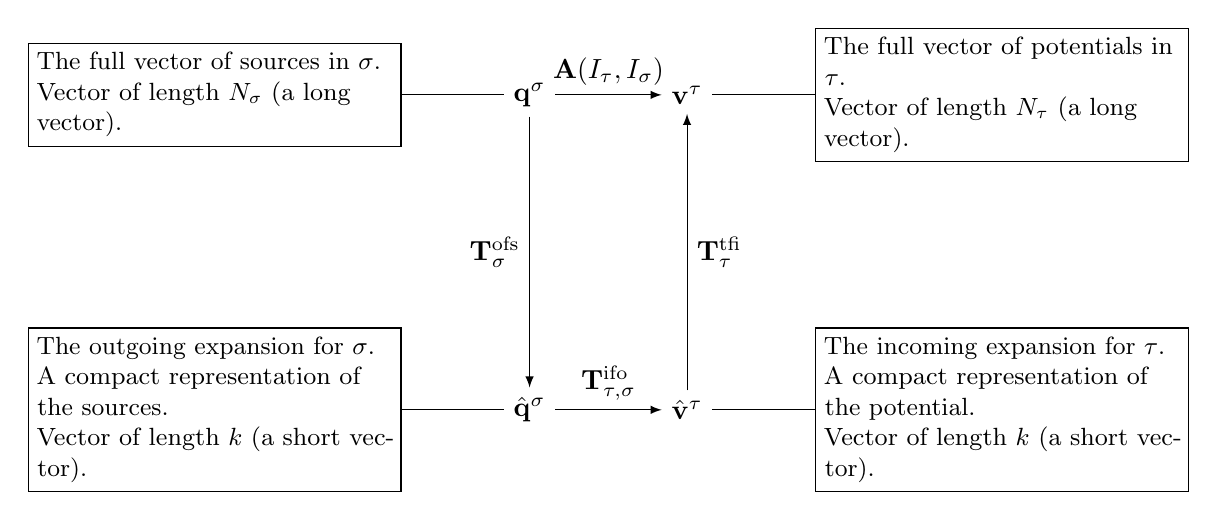
\begin{tikzpicture}[node distance=3cm and 4cm]
        % Define nodes for the vectors
        \node[draw, text width=4.5cm, align=left, font=\small] (q) at (-4, 2) {The full vector of sources in $\sigma$.\\ Vector of length $N_\sigma$ (a long vector).};
        \node[draw, text width=4.5cm, align=left, font=\small] (v) at (6, 2) {The full vector of potentials in $\tau$.\\ Vector of length $N_\tau$ (a long vector).};
        \node[draw, text width=4.5cm, align=left, font=\small] (qhat) at (-4, -2) {The outgoing expansion for $\sigma$.\\ A compact representation of the sources.\\ Vector of length $k$ (a short vector).};
        \node[draw, text width=4.5cm, align=left, font=\small] (vhat) at (6, -2) {The incoming expansion for $\tau$.\\ A compact representation of the potential.\\ Vector of length $k$ (a short vector).};

        % Define intermediate nodes
        \node (qmid) at (0, 2) {$\mathbf{q}^\sigma$};
        \node (vmid) at (2, 2) {$\mathbf{v}^\tau$};
        \node (qhatmid) at (0, -2) {$\hat{\mathbf{q}}^\sigma$};
        \node (vhatmid) at (2, -2) {$\hat{\mathbf{v}}^\tau$};

        % Draw arrows
        \draw[-latex] (qmid) -- (vmid) node[midway, above] {$\mathbf{A}(I_\tau, I_\sigma)$};
        \draw[-latex] (qmid) -- (qhatmid) node[midway, left] {$\mathbf{T}_\sigma^{\text{ofs}}$};
        \draw[-latex] (qhatmid) -- (vhatmid) node[midway, above] {$\mathbf{T}_{\tau,\sigma}^{\text{ifo}}$};
        \draw[-latex] (vhatmid) -- (vmid) node[midway, right] {$\mathbf{T}_\tau^{\text{tfi}}$};

        % Draw lines from boxes to intermediate nodes
        \draw (q) -- (qmid);
        \draw (v) -- (vmid);
        \draw (qhat) -- (qhatmid);
        \draw (vhat) -- (vhatmid);
    \end{tikzpicture}
    }
    \caption{Ilustración del flujo de información en el FMM:\ fuentes originales ($\mathbf{q}^\sigma$) $\rightarrow$ expansión saliente ($\hat{\mathbf{q}}^\sigma$) $\rightarrow$ expansión entrante ($\hat{\mathbf{v}}^\tau$) $\rightarrow$ potenciales ($\mathbf{v}^\tau$), mostrando los operadores T\textsuperscript{ofs}, T\textsuperscript{ifo}, y T\textsuperscript{tfi}. Adaptado de~\cite{Martinsson2012}.}%
    \label{fig:fmm_translations}
\end{figure}


\subsection{Contexto Histórico/Origen}

El FMM fue introducido formalmente por Leslie Greengard y Vladimir Rokhlin en su seminal artículo de 1987~\cite{GreengardRokhlin1987}, aunque ideas relacionadas con expansiones multipolares y métodos jerárquicos existían previamente (e.g.,~\cite{Appel1985, BarnesHut1986}). El trabajo de Greengard y Rokhlin proporcionó un marco riguroso y un algoritmo con complejidad demostrada de $O(N)$ para el problema de Laplace, revolucionando la simulación de $N$-cuerpos y la solución de ecuaciones integrales~\cite{GreengardRokhlin1987}. Su impacto fue tal que fue incluido en la lista de los 10 algoritmos más importantes del siglo XX~\cite{Cipra2000}.

\subsection{Variantes o Enfoques Principales}

El FMM ha evolucionado considerablemente desde su concepción original:
\begin{itemize}
    \item \textbf{Extensiones a otros Kernels:} Aunque inicialmente formulado para el kernel de Laplace ($1/r$), se ha extendido a otros kernels importantes como el de Helmholtz (ondas), Stokes (fluidos), Yukawa (física de partículas) y elasticidad~\cite{ChengEtAl1999, Martinsson2012, Rokhlin1990}. Para kernels oscilatorios como el de Helmholtz, se requieren enfoques más sofisticados (e.g., \textit{FMM direccional}) para mantener la eficiencia, especialmente a altas frecuencias~\cite{EngquistYing2009, Rokhlin1990}.
    \item \textbf{Métodos Adaptativos:} Para manejar distribuciones de partículas altamente no uniformes, se desarrollaron versiones adaptativas del FMM que refinan el árbol jerárquico solo donde es necesario, manteniendo la eficiencia~\cite{CarrierEtAl1988, ChengEtAl1999}.
    \item \textbf{FMM Independiente del Kernel (KIFMM):} Estos métodos buscan separar la maquinaria del FMM (árbol, traslaciones) de las expansiones específicas del kernel, utilizando representaciones intermedias como cargas equivalentes/ficticias y potenciales de chequeo, lo que facilita su aplicación a nuevos kernels~\cite{YingEtAl2004, Martinsson2012}.
    \item \textbf{Optimizaciones para Baja Precisión:} En campos como la astrofísica, donde no siempre se requiere alta precisión, se han desarrollado métodos FMM-like o variantes de códigos de árbol optimizados, que pueden lograr complejidades $O(N)$ o incluso sublineales empíricamente~\cite{Dehnen2002}. El método de Dehnen~\cite{Dehnen2002}, por ejemplo, utiliza interacciones celda-celda y expansiones de Taylor, conservando el momento lineal.
    \item \textbf{Versiones Paralelas y para GPU:} Se han desarrollado implementaciones altamente optimizadas para arquitecturas paralelas modernas, incluyendo CPUs multi-núcleo y GPUs, lo que permite abordar problemas de escala masiva~\cite{YokotaBarba2012, Martinsson2012}.
\end{itemize}

\subsection{Aplicaciones Típicas}

El FMM es una herramienta esencial en:
\begin{itemize}
    \item \textbf{Astrofísica:} Simulación de la evolución dinámica de galaxias y cúmulos estelares (interacciones gravitacionales)~\cite{Dehnen2002, Cipra2000}.
    \item \textbf{Dinámica Molecular:} Cálculo de fuerzas electrostáticas y de van der Waals en simulaciones de proteínas y otras biomoléculas~\cite{BeatsonGreengard1997}.
    \item \textbf{Electromagnetismo:} Solución de ecuaciones integrales para el cálculo de capacitancia, dispersión de ondas electromagnéticas y diseño de antenas~\cite{ChengEtAl1999, Martinsson2012}.
    \item \textbf{Mecánica de Fluidos:} Simulación de flujos utilizando métodos de vórtices o resolviendo ecuaciones integrales para flujos de Stokes~\cite{BeatsonGreengard1997}.
    \item \textbf{Método de Elementos de Contorno (BEM):} Aceleración de la solución de sistemas lineales densos que surgen de la discretización de ecuaciones integrales de contorno~\cite{ChenSF, Martinsson2012}.
\end{itemize}

\subsection{Ventajas y Desventajas/Limitaciones}

\textbf{Ventajas:}
\begin{itemize}
    \item \textbf{Eficiencia Asintótica:} Su complejidad $O(N)$ o $O(N \log N)$ lo hace significativamente más rápido que los métodos directos $O(N^2)$ para $N$ grande~\cite{GreengardRokhlin1987}.
    \item \textbf{Precisión Controlable:} La exactitud de la aproximación se puede ajustar sistemáticamente aumentando el orden $p$ de las expansiones~\cite{BeatsonGreengard1997}.
    \item \textbf{Escalabilidad:} Las versiones modernas han demostrado una excelente escalabilidad en arquitecturas paralelas de alto rendimiento~\cite{YokotaBarba2012}.
    \item \textbf{Amplia Aplicabilidad:} Existen variantes para una gran diversidad de kernels de interacción física~\cite{Martinsson2012}.
\end{itemize}

\textbf{Desventajas/Limitaciones:}
\begin{itemize}
    \item \textbf{Complejidad de Implementación:} El algoritmo es considerablemente más complejo de implementar y depurar que los métodos directos o códigos de árbol más simples~\cite{BeatsonGreengard1997, Martinsson2012}.
    \item \textbf{Constante Oculta:} Aunque asintóticamente eficiente, la constante multiplicativa en la complejidad $O(N)$ puede ser grande, haciendo que para valores pequeños o intermedios de $N$, métodos más simples (como Barnes-Hut o incluso directos) puedan ser competitivos~\cite{Dehnen2002}.
    \item \textbf{Consumo de Memoria:} Requiere almacenar las expansiones multipolares y locales en cada celda del árbol, lo que puede incrementar el uso de memoria en comparación con métodos directos~\cite{YingEtAl2004}.
    \item \textbf{Rendimiento en Distribuciones No Uniformes:} Las versiones no adaptativas pueden perder eficiencia si la distribución de partículas es muy irregular, aunque las variantes adaptativas mitigan este problema~\cite{CarrierEtAl1988, ChengEtAl1999}.
\end{itemize}

% --- Placeholder para Tabla (Comparación Complejidad) ---
\begin{table}[H]
    \centering
    \caption{Comparación de complejidad computacional para problemas de N-cuerpos.}%
    \label{tab:fmm_complexity}
    \begin{tabular}{lc}
        \hline % chktex 44
        \textbf{Método} & \textbf{Complejidad Computacional} \\
        \hline % chktex 44
        Cálculo Directo & $O(N^2)$ \\
        Algoritmo Barnes-Hut & $O(N \log N)$ \\
        Método Multipolar Rápido (FMM) & $O(N)$ o $O(N \log N)$ \\
        % FMM (Estimación precisa, d dims) & $O(N \log^{(d-1)}(1/\epsilon))$ \\ % Opcional
        \hline % chktex 44
    \end{tabular}\\
    \medskip \small Fuente: Basado en~\cite{GreengardRokhlin1987, BeatsonGreengard1997, Martinsson2012}.
\end{table}

    \subsection{Simulación Barnes-Hut}%
\label{sec:barnes_hut}

La simulación Barnes-Hut es un algoritmo de aproximación ampliamente utilizado en el campo de la física computacional, especialmente en astrofísica, para simular la evolución dinámica de sistemas de N-cuerpos (\textit{N-body systems}) bajo la influencia de fuerzas de largo alcance, como la gravedad o las interacciones electrostáticas~\cite{Barnes1986, dubinski1996}. Fue propuesto originalmente por Josh Barnes y Piet Hut en 1986~\cite{Barnes1986} como una solución eficiente al problema computacionalmente intensivo del cálculo directo de todas las interacciones por pares en un sistema grande, cuya complejidad escala como $O(N^2)$. El algoritmo Barnes-Hut reduce esta complejidad a $O(N \log N)$, permitiendo la simulación de sistemas con un número significativamente mayor de partículas~\cite{Barnes1986, salmon1991}.

\subsubsection{Principios y Funcionamiento}

El principio fundamental del algoritmo Barnes-Hut radica en la aproximación de la fuerza ejercida por un grupo distante de partículas tratándolo como una única pseudo-partícula (o un conjunto de momentos multipolares de bajo orden) ubicada en el centro de masa (CoM) del grupo~\cite{Barnes1986, barnes1990}. Esta aproximación es válida porque el campo gravitatorio (o electrostático) de un grupo de partículas a gran distancia se asemeja al de una sola partícula puntual con la masa total del grupo ubicada en su centro de masa~\cite{pfalzner1996}.

Para implementar esta idea, el algoritmo emplea una estructura de datos jerárquica basada en la subdivisión recursiva del espacio:

\begin{enumerate}
    \item \textbf{Construcción del Árbol (\textit{Tree Construction}):} El espacio que contiene las N partículas se subdivide recursivamente en celdas. En 3D, se utiliza un \textit{octree} (árbol óctuple), donde el cubo que engloba todo el sistema se divide en ocho subcubos (octantes) iguales. Este proceso se repite para cada subcubo que contenga más de una partícula, hasta que cada celda hoja (nodo terminal del árbol) contenga como máximo una partícula~\cite{Barnes1986, dubinski1996}. En 2D, se utiliza una estructura análoga llamada \textit{quadtree} (árbol cuádruple)~\cite{aguirre2020, munier2020}. Cada nodo interno del árbol almacena información agregada sobre las partículas contenidas en su celda correspondiente, como la masa total y la posición del centro de masa~\cite{Barnes1986, salmon1991}.

    \item \textbf{Cálculo de Fuerzas (\textit{Force Calculation}):} Para calcular la fuerza neta sobre una partícula específica $i$, se recorre el árbol desde la raíz. Para cada nodo (celda) $c$ encontrado durante el recorrido, se aplica el \textit{criterio de apertura de Barnes-Hut} (\textit{Barnes-Hut opening criterion}). Este criterio compara el tamaño de la celda $s$ (usualmente su anchura o diagonal) con la distancia $d$ entre la partícula $i$ y el centro de masa de la celda $c$. Si la relación $s/d$ es menor que un parámetro de precisión umbral $\theta$ (theta), es decir:
    \[ s / d < \theta \]
    la celda $c$ se considera ``suficientemente lejana''. En este caso, la contribución a la fuerza sobre la partícula $i$ debida a todas las partículas dentro de la celda $c$ se aproxima utilizando la masa total y el centro de masa (o una expansión multipolar de bajo orden) almacenados en el nodo $c$~\cite{Barnes1986, salmon1991, barnes1990}. Si la condición no se cumple ($s/d \ge \theta$), la celda está demasiado cerca o es demasiado grande para ser aproximada con precisión, por lo que el algoritmo desciende recursivamente a los hijos de ese nodo (si es un nodo interno) y repite el proceso~\cite{Barnes1986, barnes1990}. Si el nodo es una hoja que contiene una partícula $j$ (distinta de $i$), la fuerza entre $i$ y $j$ se calcula directamente~\cite{pfalzner1996}. El valor de $\theta$ (típicamente entre 0.5 y 1.2) controla el equilibrio entre precisión y velocidad: valores más pequeños de $\theta$ resultan en cálculos más precisos pero más lentos (más interacciones directas y nodos visitados), mientras que valores más grandes aceleran el cálculo a costa de una menor precisión~\cite{barnes1990, aguirre2020}.
\end{enumerate}

\subsubsection{Contexto Histórico y Origen}

El algoritmo fue presentado por Josh Barnes y Piet Hut en su artículo de 1986 en la revista \textit{Nature}, titulado ``A hierarchical $O(N \log N)$ force-calculation algorithm''~\cite{Barnes1986}. Su desarrollo fue motivado por la necesidad de superar las limitaciones computacionales de las simulaciones N-cuerpos directas en astrofísica, que impedían estudiar sistemas a gran escala como la formación y dinámica de galaxias o cúmulos estelares~\cite{Barnes1986, dubinski1996}. El algoritmo Barnes-Hut representó un avance significativo al hacer factibles simulaciones con cientos de miles o millones de partículas en la época.

\subsubsection{Variantes y Enfoques Principales}

Desde su concepción, el algoritmo Barnes-Hut ha sido objeto de diversas optimizaciones y variantes:

\begin{itemize}
    \item \textbf{Implementaciones Paralelas:} Dada la naturaleza jerárquica y divisible del problema, el algoritmo se adapta bien a la paralelización. Se han desarrollado diversas estrategias para distribuir la construcción del árbol y el cálculo de fuerzas entre múltiples procesadores o nodos de cómputo, utilizando técnicas como la descomposición de dominio (ej.\ \textit{Bisección Recursiva Ortogonal \- ORB}~\cite{salmon1991}) o la distribución de partículas basada en carga computacional~\cite{dubinski1996, becciani1997, becciani2000}.
    \item \textbf{Aceleración por GPU:} Las unidades de procesamiento gráfico (GPUs), con su arquitectura masivamente paralela, han demostrado ser muy eficaces para acelerar las simulaciones Barnes-Hut~\cite{burtscher2011, hamada2009}. Existen implementaciones donde partes significativas o la totalidad del algoritmo se ejecutan en la GPU~\cite{burtscher2011}.
    \item \textbf{Expansiones Multipolares:} Para mejorar la precisión de la aproximación de fuerzas de grupos distantes, en lugar de usar solo el monopolo (masa total y CoM), se pueden incluir términos de orden superior como el cuadrupolo~\cite{barnes1990, salmon1994}. Esto es especialmente relevante cuando se requiere una alta fidelidad en la simulación.
    \item \textbf{Combinación con otros Métodos:} En algunas simulaciones cosmológicas a gran escala, el algoritmo Barnes-Hut puede combinarse con métodos de malla de partículas (\textit{Particle-Mesh}, PM) para manejar las fuerzas de largo alcance de manera eficiente, mientras que Barnes-Hut se encarga de las interacciones a corta y mediana escala~\cite{bagla2004}.
    \item \textbf{Optimización de Árboles:} Se han explorado variantes en la construcción y recorrido del árbol, como los árboles \textit{k-d} o el uso de árboles duales (\textit{dual-tree}) que recorren simultáneamente dos árboles para optimizar el cálculo de interacciones celda-celda en lugar de partícula-celda~\cite{vandemaaten2008, vandermaaten2013}.
\end{itemize}

\subsubsection{Aplicaciones Típicas}

El algoritmo Barnes-Hut y sus variantes se aplican en diversos campos científicos y técnicos:

\begin{itemize}
    \item \textbf{Astrofísica:} Es una herramienta estándar para simulaciones de formación y evolución de galaxias, interacciones galácticas, dinámica de cúmulos estelares y globulares, y formación de estructuras a gran escala en cosmología~\cite{dubinski1996, salmon1991, bagla2004}.
    \item \textbf{Dinámica Molecular:} Se utiliza para calcular eficientemente las interacciones electrostáticas y de Van der Waals (que también son de largo alcance) en simulaciones de sistemas moleculares grandes como proteínas, ADN o fluidos iónicos~\cite{pfalzner1996, Gan2014}.
    \item \textbf{Física de Plasmas:} Para simular la interacción entre partículas cargadas en plasmas~\cite{winkel2012}.
    \item \textbf{Visualización de Datos y Aprendizaje Automático:} Se ha adaptado para acelerar algoritmos de reducción de dimensionalidad y visualización, como t-SNE (\textit{t-distributed Stochastic Neighbor Embedding}), donde se modelan ``fuerzas'' atractivas y repulsivas entre puntos de datos en un espacio de baja dimensión~\cite{vandemaaten2008, vandermaaten2013}.
    \item \textbf{Graficación por Computadora y Diseño de Grafos:} Para algoritmos de diseño dirigido por fuerzas (\textit{force-directed layout}), donde los nodos de un grafo se repelen y las aristas actúan como resortes, buscando una disposición espacial estéticamente agradable o funcional~\cite{Nguyen2007}.
\end{itemize}

\subsubsection{Ventajas y Limitaciones}

\paragraph{Ventajas}
\begin{itemize}
    \item \textbf{Eficiencia Computacional:} Su complejidad $O(N \log N)$ permite simular sistemas mucho más grandes que los métodos directos $O(N^2)$~\cite{Barnes1986}.
    \item \textbf{Versatilidad:} Aplicable a diferentes tipos de fuerzas de largo alcance (gravitatoria, electrostática)~\cite{pfalzner1996, Gan2014}.
    \item \textbf{Adaptabilidad:} La estructura de árbol se adapta naturalmente a distribuciones de partículas no uniformes (clusterizadas)~\cite{becciani1997, dubinski1996}.
    \item \textbf{Paralelizable:} Se presta bien a la implementación en arquitecturas de cómputo paralelo (multi-núcleo, GPU, clusters)~\cite{dubinski1996, burtscher2011}.
\end{itemize}

\paragraph{Limitaciones}
\begin{itemize}
    \item \textbf{Aproximación:} Introduce errores en el cálculo de fuerzas, cuya magnitud depende del parámetro $\theta$ y de la distribución de partículas~\cite{barnes1990, aguirre2020}. No es adecuado para simulaciones que requieran una precisión extremadamente alta en las interacciones individuales (ej.\ dinámica de sistemas planetarios precisos a largo plazo).
    \item \textbf{Complejidad de Implementación:} Aunque conceptualmente más simple que otros métodos rápidos como el Método Multipolo Rápido (FMM), su implementación correcta, especialmente las versiones paralelas u optimizadas, requiere un esfuerzo considerable~\cite{dubinski1996, salmon1991}.
    \item \textbf{Coste de Construcción del Árbol:} La construcción (o reconstrucción) del árbol en cada paso de tiempo representa una sobrecarga computacional que no existe en los métodos directos~\cite{salmon1991}.
    \item \textbf{Condiciones de Contorno:} La implementación de condiciones de contorno periódicas, comunes en cosmología o dinámica molecular, es más compleja que en métodos basados en mallas~\cite{bagla2004}.
\end{itemize}

    \section[REBOUND]{REBOUND:\ Código N-cuerpos multipropósito de código abierto para dinámica colisional}

REBOUND (Rein \& Liu, 2012)~\cite{Rein2012} se define como un código numérico de N-cuerpos, multipropósito y de código abierto, distribuido bajo la licencia GPLv3~\cite{Rein2012}. Fue diseñado primordialmente para abordar problemas de dinámica colisional, como los encontrados en anillos planetarios, pero es igualmente capaz de resolver el problema clásico de N-cuerpos en sistemas puramente gravitacionales~\cite{Rein2012} [Abstract, Sec. 1]. Su desarrollo buscó llenar un vacío existente en cuanto a códigos públicos disponibles para la simulación de dinámica colisional compleja~\cite{Rein2012} [Sec. 1].

\subsection{Principios Fundamentales y Funcionamiento}

La filosofía central de REBOUND es su alta modularidad~\cite{Rein2012} [Abstract, Sec. 2.2]. Está escrito enteramente en C (conforme al estándar ISO C99) y diseñado para compilar y ejecutarse en plataformas modernas compatibles con POSIX (como Linux, Unix y Mac OSX)~\cite{Rein2012} [Sec. 2, Sec. 2.1]. La estructura modular permite al usuario seleccionar y combinar diferentes componentes mediante el uso de enlaces simbólicos, sin necesidad de modificar el código fuente principal. Esto facilita la adaptación del código a una amplia variedad de problemas astrofísicos y de otras disciplinas~\cite{Rein2012} [Sec. 2.2]. Los módulos intercambiables incluyen:

\begin{enumerate}
    \item \textbf{Integradores Numéricos:} REBOUND implementa varios integradores, mayormente basados en el esquema simpléctico de segundo orden Drift-Kick-Drift (DKD). Es importante notar que la naturaleza simpléctica se pierde formalmente si se introducen aproximaciones en el cálculo de la gravedad, colisiones o fuerzas dependientes de la velocidad~\cite{Rein2012} [Sec. 3]. Los integradores principales son:
    \begin{itemize}
        \item \textbf{Leap-frog:} Un integrador simpléctico estándar de segundo orden para marcos no rotacionales~\cite{Rein2012} [Sec. 3.1].
        \item \textbf{Wisdom-Holman (WH):} Un mapeo simpléctico de variables mixtas que integra el movimiento kepleriano de forma exacta durante el paso de deriva (\textit{drift}). Es muy preciso para problemas dominados por un potencial central $1/r$, pero computacionalmente más costoso que Leap-frog debido a la resolución iterativa de la ecuación de Kepler~\cite{Rein2012} [Sec. 3.2].
        \item \textbf{Symplectic Epicycle Integrator (SEI):} Diseñado para la aproximación de Hill (utilizada en láminas de cizallamiento o \textit{shearing sheets}), opera en un marco rotacional y es computacionalmente rápido~\cite{Rein2012} [Sec. 3.3].
    \end{itemize}
    REBOUND utiliza un paso de tiempo (\textit{timestep}) fijo para todas las partículas por defecto, lo cual es crucial para mantener las propiedades simplécticas de los integradores correspondientes. Es responsabilidad del usuario asegurar que el paso de tiempo sea suficientemente pequeño para la convergencia numérica~\cite{Rein2012} [Sec. 3].

    \item \textbf{Cálculo de Gravedad:} Se proporcionan dos módulos principales para calcular las fuerzas gravitacionales~\cite{Rein2012} [Sec. 4]:
    \begin{itemize}
        \item \textbf{Suma Directa:} Calcula la interacción entre todos los pares de partículas activas ($N_{\text{active}}$) de forma exacta (ecuación 1 en~\cite{Rein2012}). Su costo computacional escala como $O(N \cdot N_{\text{active}})$, siendo eficiente solo para un número bajo de partículas masivas ($N_{\text{active}} \le 10^2$)~\cite{Rein2012} [Sec. 4.1]. Permite incluir un parámetro de suavizado gravitacional ($b$) para evitar aceleraciones extremas en encuentros cercanos~\cite{Rein2012} [Eq. 1].
        \item \textbf{Octree (Árbol Octal):} Implementa el algoritmo de Barnes \& Hut (1986) para aproximar las fuerzas de largo alcance, reduciendo la complejidad computacional a $O(N \log N)$~\cite{Rein2012} [Sec. 4.2]. Agrupa jerárquicamente las partículas distantes y utiliza su centro de masa (y opcionalmente su tensor cuadrupolar, siguiendo a Hernquist, 1987) para calcular la fuerza, basándose en un criterio de ángulo de apertura ($\theta_{\text{crit}}$). Este módulo está completamente paralelizado usando MPI (con descomposición estática de dominio y árboles esenciales distribuidos) y OpenMP~\cite{Rein2012} [Sec. 4.2, Sec. 7].
        % Sugerencia Visual:
        % [Aquí podría insertarse una figura adaptada de la Fig. 4 de~\cite{Rein2012} para ilustrar la convergencia
        % de la precisión de la fuerza en función de theta_crit y la mejora al incluir el término cuadrupolar].
    \end{itemize}

    \item \textbf{Detección de Colisiones:} REBOUND incluye varios módulos para detectar colisiones, modeladas como interacciones entre esferas duras con un coeficiente de restitución $\epsilon$ especificado por el usuario~\cite{Rein2012} [Sec. 5]. Las colisiones detectadas en un paso de tiempo se resuelven en orden aleatorio para evitar sesgos~\cite{Rein2012} [Sec. 5]. Los métodos son:
    \begin{itemize}
        \item \textbf{Búsqueda Directa del Vecino Más Cercano:} Comprueba el solapamiento de todas las parejas de partículas al final del paso de tiempo. Escala como $O(N^2)$~\cite{Rein2012} [Sec. 5.1].
        \item \textbf{Octree:} Utiliza la estructura del árbol octal para buscar vecinos cercanos y detectar solapamientos, con una complejidad promedio de $O(N \log N)$. Puede usar la misma estructura del árbol de gravedad y está paralelizado (MPI/OpenMP)~\cite{Rein2012} [Sec. 5.2].
        \item \textbf{Algoritmo de Barrido Plano (Plane-Sweep):} Dos variantes (cartesiana en $x$ y angular en $\phi$) basadas en el algoritmo de Bentley \& Ottmann (1979), pero simplificadas. Aproxima las trayectorias de las partículas como líneas rectas durante un paso de tiempo. Mueve un plano conceptual a través del dominio, manteniendo una lista de partículas activas intersectadas por el plano y comprobando colisiones solo dentro de esa lista. Su complejidad es $O(N \cdot N_{\text{SWEEPL}})$, donde $N_{\text{SWEEPL}}$ es el número promedio de partículas en la lista activa. Es significativamente más eficiente que los métodos basados en árboles para simulaciones cuasi-bidimensionales o muy elongadas (donde $N_{\text{SWEEPL}}$ es pequeño), como anillos planetarios densos o simulaciones en láminas de cizallamiento~\cite{Rein2012} [Sec. 5.3].
        \begin{figure}[H]
            \centering
            % Descomenta la siguiente línea e inserta la ruta a tu imagen
            \includegraphics[width=\textwidth]{img/marcoTeorico/Algoritmo_de_barrido_plano.png}
            %\fbox{\parbox{0.8\textwidth}{\centering Placeholder: Figura Esquema de la Jerarquía de Celdas y Listas de Interacción}}
            \caption{Ilustración del algoritmo de barrido plano. El plano interseca las trayectorias de las partículas 5 y 7. Véanse los detalles en el texto adaptado de~\cite{Rein2012}.}%
            \label{fig:plane_sweep_algorithm}
        \end{figure}
    \end{itemize}

    \item \textbf{Condiciones de Contorno:} Soporta condiciones de contorno abiertas (las partículas que salen son eliminadas), periódicas (implementadas con cajas fantasma) y de lámina de cizallamiento (\textit{shear-periodic})~\cite{Rein2012} [Sec. 2.3].
\end{enumerate}

\subsection{Contexto Histórico y Origen}

El código fue presentado por H. Rein y S.-F. Liu en 2012~\cite{Rein2012}, aunque versiones precursoras ya se habían utilizado en publicaciones anteriores (e.g., Rein \& Papaloizou, 2010; Crida et al., 2010; Rein et al., 2010)~\cite{Rein2012} [Sec. 1]. Nació de la necesidad de contar con una herramienta pública, flexible y eficiente para estudiar la dinámica de sistemas astrofísicos donde las colisiones juegan un papel crucial, como los anillos de Saturno o los discos protoplanetarios~\cite{Rein2012} [Sec. 1].

\subsection{Variantes y Enfoques Principales}

Más que variantes distintas del código, REBOUND ofrece diferentes enfoques de simulación a través de la combinación de sus módulos. El usuario puede configurar la simulación eligiendo el integrador más adecuado (e.g., WH para alta precisión a largo plazo en sistemas planetarios, SEI para láminas de cizallamiento, Leap-frog como opción general), el método de cálculo de gravedad (directo para pocos cuerpos, árbol para muchos) y el algoritmo de detección de colisiones (directo, árbol, o barrido plano según la geometría y densidad del problema)~\cite{Rein2012} [Sec. 2.2, Sec. 3, Sec. 4, Sec. 5].

\subsection{Aplicaciones Típicas}

La literatura documenta el uso de REBOUND en una variedad de problemas astrofísicos:
\begin{itemize}
    \item Simulación de anillos planetarios, incluyendo el estudio de su viscosidad y estructuras inducidas por satélites~\cite{Rein2012} [Sec. 1, Sec. 6.4].
    \item Formación de planetesimales a partir de enjambres de partículas en discos protoplanetarios~\cite{Rein2012} [Sec. 1].
    \item Estudio de discos de transición y de escombros (utilizando superpartículas)~\cite{Rein2012} [Sec. 1].
    \item Problemas clásicos de N-cuerpos, como la integración a largo plazo de la dinámica del Sistema Solar~\cite{Rein2012} [Sec. 1, Sec. 6.3].
\end{itemize}
Aunque diseñado para astrofísica, su estructura modular lo hace potencialmente aplicable a otros campos que involucren dinámica de partículas, como la dinámica molecular o flujos granulares~\cite{Rein2012} [Abstract].

\subsection{Ventajas y Limitaciones}

Las principales \textbf{ventajas} de REBOUND, según se desprenden de~\cite{Rein2012}, son:
\begin{itemize}
    \item \textbf{Código Abierto y Gratuito:} Accesible para la comunidad científica bajo licencia GPLv3~\cite{Rein2012} [Sec. 1].
    \item \textbf{Modularidad y Flexibilidad:} Altamente personalizable para diferentes problemas~\cite{Rein2012} [Abstract, Sec. 2.2].
    \item \textbf{Eficiencia y Escalabilidad:} Demuestra buen escalado en paralelo (tanto fuerte como débil) usando MPI y OpenMP, permitiendo simulaciones con un gran número de partículas en clústeres de cómputo~\cite{Rein2012} [Abstract, Sec. 7].
    \item \textbf{Variedad de Métodos:} Ofrece múltiples opciones de integradores, cálculo de gravedad y detección de colisiones~\cite{Rein2012} [Sec. 3, Sec. 4, Sec. 5].
    \item \textbf{Precisión:} Los integradores simplécticos son adecuados para integraciones a largo plazo, y se conserva la energía y el momento hasta la precisión de la máquina en colisiones elásticas~\cite{Rein2012} [Sec. 3, Sec. 6.2].
\end{itemize}

Las \textbf{limitaciones} inherentes o aspectos a considerar son:
\begin{itemize}
    \item \textbf{Paso de Tiempo Fijo:} Generalmente requerido por los integradores simplécticos, lo que puede ser ineficiente si ocurren escalas de tiempo muy diferentes en el sistema~\cite{Rein2012} [Sec. 3]. El usuario debe elegirlo cuidadosamente.
    \item \textbf{Pérdida de Simplecticidad:} Las propiedades simplécticas se pierden si se usan aproximaciones (árbol de gravedad), colisiones o fuerzas no conservativas~\cite{Rein2012} [Sec. 3].
    \item \textbf{Aproximaciones:} Los métodos de árbol para gravedad y colisiones son aproximados, con una precisión que depende de parámetros como $\theta_{\text{crit}}$~\cite{Rein2012} [Sec. 4.2, Sec. 6.1]. El método de barrido plano aproxima las trayectorias como líneas rectas entre pasos~\cite{Rein2012} [Sec. 5.3, Fig. 2].
    \item \textbf{Rendimiento:} El rendimiento del árbol puede degradarse si el número de partículas por nodo MPI es muy bajo debido al costo de comunicación~\cite{Rein2012} [Sec. 7.1]. La eficiencia del barrido plano depende crucialmente de la dimensionalidad efectiva del problema~\cite{Rein2012} [Sec. 5.3, Sec. 9].
\end{itemize}


    \appendix
        %\include{Appendices/appendixA}
        %\include{Appendices/appendixB}

\backmatter%
    \bookmarksetup{startatroot}
    \printbibliography[heading=bibintoc]
\end{document}